\documentclass[11pt,a4paper,oneside]{book}

\usepackage[dutch]{babel}
\usepackage{blindtext}

\usepackage[backend=biber, style=ieee,natbib=true]{biblatex}
\addbibresource{references.bib}

\usepackage[plainpages=false]{hyperref}    % Om hyperlinks te hebben in het pdfdocument.
\usepackage{a4wide}
\usepackage{url}

\usepackage[T1]{fontenc}

\usepackage{dirtree}

\usepackage{minted}
\setminted{frame=single,framesep=3mm,linenos}

\usepackage{csquotes}
\usepackage{wrapfig}
\usepackage{graphicx}
\graphicspath{./figures/}

\usepackage[parfill]{parskip}

\usepackage[small,bf,hang]{caption2}


\author{Branco Bruyneel}
\title{Wat is de huidige status van Rust voor het bouwen van webapplicaties?}

\begin{document}

\maketitle

\chapter*{Woord vooraf}
Ter afsluiting van mijn opleiding New Media \& Creative Technologies aan de Hogeschool
West-Vlaanderen te Kortrijk, schreef ik deze bachelorproef.  In het 4e semester van deze opleiding
koos ik ‘AI Engineer’ als uitstromingsprofiel. Een semester later, koos ik bij de module ‘Research
Project’ een onderzoeksvraag die niks te maken heeft met Artificiële Intelligentie. De
onderzoeksvraag luidt als volgt: “Wat is de huidige status van Rust voor het bouwen van
webapplicaties?” en is dan ook het onderwerp voor deze bachelorproef. 

Deze bachelorproef bespreekt eerst de research en technische demo uit de module ‘Research Project’.
De demo bestond uit een speed typing test applicatie, waar een gebruiker zo snel mogelijk een random
code fragment moet over typen om erna zijn prestaties te kunnen bekijken. 

Na de analyse reflecteer ik het verkregen resultaat met het werkveld. Hiervoor nam ik contact op met
een van de core maintainers van Yew genaamd Julius Lungys en Industrieel Ingenieur Emiel Van
Severen. Op basis hiervan volgt een vrijblijvend advies voor bedrijven. 

Graag bedank ik Stijn Walcarius die mij de kans gaf om dit onderzoek te mogen uitvoeren sinds deze
onderzoeksvraag bestemd was voor een ander uitstromingsprofiel. Waardoor ik met plezier een nieuwe
programmeertaal heb ontdekt en het ook meteen mijn favoriete taal is geworden. 

Tot slot bedank ik Niek Candaele en Jonas De Meyer voor het nalezen en constructieve feedback op
deze bachelorproef.

\chapter*{Abstract}
Samenvatting of abstract (mag in het Engels): MAX 1 halve A4-pagina:  

Je beantwoordt in de samenvatting kort en bondig een viertal vragen:  
\begin{itemize}
  \item Wat is de onderzoeksvraag? 
  \item Wat was jouw onderzoek?  
  \item Welke elementen spelen een grote rol (zowel positief als negatief) bij de evaluatie van het
    onderzoek?  
  \item Welke elementen zijn belangrijk bij jouw advies? 
  \item Het besluit wordt kort samengevat.
\end{itemize}

\tableofcontents
\addcontentsline{toc}{chapter}{Woord vooraf}
\addcontentsline{toc}{chapter}{Abstract}
\addcontentsline{toc}{chapter}{Lijst van figuren}
\addcontentsline{toc}{chapter}{Lijst met afkortingen}
\addcontentsline{toc}{chapter}{Verklarende woordenlijst}

\listoffigures

\chapter*{Lijst met afkortingen}
\chapter*{Verklarende woordenlijst}


\chapter{Inleiding}

focus op frontend / wasm

\chapter{Research}
\label{research}

\section{Wat is Rust?}

Rust is een gecompileerde multi-paradigma programmeertaal bedacht door Graydon Hoare en is begonnen
als een project van Mozilla Research. Geïnspireerd door de programmeertalen C en C++, maar kent
weinig syntactische en semantische gelijkenissen tegenover deze talen. Rust focust zich met name op
snelheid, veiligheid, betrouwbaarheid en productiviteit. Dit wordt gerealiseerd door gebruik te
maken van een krachtig typesysteem en een borrow checker. Hiermee kan Rust een hoog niveau van
geheugenveiligheid garanderen zonder een garbage collector nodig te hebben. Rust beoogt moderne
computersystemen efficiënter te benutten. Hiervoor maakt het onder meer gebruik van het ownership
systeem dat geheugen in een blok toewijst en daarnaast strikt toeziet op de stacktoewijzing.
Hierdoor kunnen problemen zoals stackoverflows, bufferoverflows en niet-geïnitialiseerd geheugen
voorkomen worden. Verder staat Rust ook geen null-pointers, dangling-pointers of data-races toe in
veilige code.

\subsection{Syntax} 

Voor velen die zich niet herkennen in programmeertalen zoals C++, Haskell of OCaml lijkt Rust een
aparte syntax te hebben in tegenstelling tot conventionele talen. Laat ons even kijken naar een paar
syntactische voorbeelden in Rust.


Hier een simpel voorbeeld dat \mintinline{rust}{"Hello world!"} schrijft naar de standaard output.

\begin{listing}[h]
\begin{minted}{rust}
fn main() {
  println!("Hello, world!");
}
\end{minted}
\caption{Hello, world!}
\end{listing}

\clearpage

Merk op dat \mintinline{rust}{println!} geen functie is maar een macro. Geïnspireerd door de
functionele programmeertaal Scheme, zijn macro’s een manier van code schrijven dat andere code
schrijft, wat bekend staat als metaprogramming. Metaprogramming is handig voor het verminderen van
code dat u zelf hoeft te schrijven en onderhouden, wat ook een van de rollen is van functies. Toch
verschillen macro’s met functies. Zo kunnen macro’s een variabel aantal parameters hebben en worden
ze uitgebreid vooraleer de compiler de betekenis van de code interpreteert.

\begin{listing}[h]
\begin{minted}{rust}
#[derive(Debug)]
struct Rectangle {
  width: u32,
  height: u32,
}

impl Rectangle {
  fn square(size: u32) -> Rectangle {
    Rectangle: {
      width: size,
      height: size,
    }
  }
  fn area(&self) -> u32 {
    self.width * self.height
  }
}

fn main() {
  let rect1 = Rectangle::square(4);
  println!(
    "The area of the rectangle is {} square pixels.",
    rect1.area()
  );
}

\end{minted}
\caption{structs}
\end{listing}

Een \mintinline{rust}{struct} in Rust is gelijkaardig als een Object in object georiënteerde
programmeertalen. Het wordt gebruikt om samenhorende waarden te groeperen en optioneel kan men
associated functions implementeren. Associated functions die geen self als hun eerste parameter
hebben zijn geen methodes en kunnen gebruikt worden als constructors die een nieuwe instantie
retourneren van de struct.

Rust heeft geen null pointers tenzij men een null pointer wil dereferentieren (dan moet die in een
\mintinline{rust}{unsafe} blok worden geplaatst). Als alternatief voor null maakt Rust gebruik van
een \mintinline{rust}{Option} type waarmee gekeken kan worden of een pointer wel
\mintinline{rust}{Some} of geen \mintinline{rust}{None} waarde bevat. Dit
kan afgehandeld worden door syntactische sugar, zoals het if let statement om toegang te krijgen tot
het innerlijke type, in dit geval een string:

\begin{listing}[h]
\begin{minted}{rust}
fn main() {
  let name: Option<String> = None;
  // If name was not None, it would print here.
  if let Some(name) = name {
    println!("{}", name);
  }
}
\end{minted}
\caption{\mintinline{rust}{Option} type}
\end{listing}

Naast de \mintinline{rust}{if} en \mintinline{rust}{else} controlestructuren is er ook match en
\mintinline{rust}{if} \mintinline{rust}{let}. match is vergelijkbaar met een
\mintinline{javascript}{switch} statement uit andere talen. Het neemt een waarde en test het tegen
een serie van patronen. Op basis van welk patroon er overeenkomt wordt de code uitgevoerd. Patronen
kunnen opgemaakt worden uit waarden, variabel namen, wildcards, en veel meer. De power van match
komt van het feit dat de compiler zal bevestigen bij het compileren dat alle mogelijke gevallen zijn
afgehandeld. Soms wil je niet alle gevallen expliciet afhandelen en wil je slechts een patroon
afhandelen terwijl je de rest negeert. In dat geval kan je \mintinline{rust}{if let} gebruiken, wat
minder boilerplate code is dan match.

\begin{listing}[h]
\begin{minted}{rust}
let message = match maybe_digit {
  Some(x) if x < 10 => process_digit(x),
  Some(x) => process_other(x),
  None => panic!(),
};

let config_max = Some(3u8);
if let Some(max) = config_max {
  println!("The maximum is configured to be {}", max);
}
\end{minted}
\caption{\mintinline{rust}{if let} \& \mintinline{rust}{match} operators}
\end{listing}

\clearpage

\subsection{Geheugen}

Bij vele programmeertalen hoef je geen zorgen te maken over het geheugen gebruik. Dit is mogelijk
door een garbage collector te gebruiken die voortdurend zoekt naar niet langer gebruikt geheugen
terwijl het programma loopt. In andere talen, moet de programmeur het geheugen expliciet toewijzen
en vrijmaken. Rust gebruikt geen van beide methodes en komt met een uniek concept genaamd ownership.
Hiermee kan het geheugen veiligheid garanderen zonder een garbage collector nodig te hebben. 

Vooraleer we verder gaan is het belangrijk dat we de twee begrippen genaamd stack en heap begrijpen.
De twee datastructuren maken deel uit van het geheugen en zijn beschikbaar voor uw code om te
gebruiken tijdens runtime, maar ze zijn op verschillende manieren gestructureerd. Wat maakt dat de
ene zorgt voor snellere dataopslag dan de andere. 

De stack slaat waarden op in de volgorde waarin hij ze krijgt en verwijdert de waarden in de
omgekeerde volgorde. Dit wordt aangeduid als last in, first out. Alle gegevens die op de stack
worden opgeslagen moeten een bekende, vaste grootte hebben. Gegevens waarvan de grootte op het
moment van compileren onbekend is of die van grootte kunnen veranderen, moeten in plaats daarvan op
de heap worden opgeslagen. 

De heap is minder georganiseerd: als je gegevens op de heap zet, vraag je een bepaalde hoeveelheid
ruimte aan. De memory allocator vindt een lege plek in de heap die groot genoeg is, markeert die als
in gebruik, en geeft een pointer terug, dat is het adres van die locatie. Dit proces wordt
'allocating on the heap' genoemd en wordt soms afgekort als gewoon allocating. Het 'pushen' van
waarden op de stack wordt niet beschouwd als allocating. Omdat de pointer naar de heap een bekende,
vaste grootte heeft, kun je de pointer op de stack opslaan, maar als je de eigenlijke gegevens wilt
hebben, moet je de pointer volgen. 

Het efficiëntste is dus om data naar de stack weg te schrijven dan naar de heap, omdat de allocator
nooit hoeft te zoeken naar een plaats om nieuwe gegevens op te slaan. Die plaats is altijd bovenaan
de stack. Het alloceren van ruimte op de heap vergt meer werk, omdat de allocator eerst een ruimte
moet vinden die groot genoeg is om de gegevens op te slaan en dan de boekhouding moet doen om de
volgende allocatie voor te bereiden. 

Rust heeft dus een voorkeur om zijn variabelen weg te schrijven naar de stack. Maar zoals gezegd kan
je niet elke variabele wegschrijven naar de stack, daarom is er een onderscheid tussen simpele en
complexe types. Bij simpele types ken je de grootte voor het compileren, daarmee worden ze dan ook
opgeslagen op de stack. In tegenstelling tot complexe types waarbij de grootte kan veranderen,
worden ze opgeslagen in de heap.

De simpele types zijn:
\begin{itemize}
  \item Integer
  \item Floating-point
  \item Boolean
  \item Character
  \item Tuple
  \item Array (ze hebben dus een vaste grootte in Rust)
\end{itemize}

Nu de begrippen zijn opgeklaard kunnen we kijken naar het ownership systeem. Het systeem bestaat uit
drie regels: 
\begin{enumerate}
  \item Elke waarde in Rust heeft een variabele die de owner wordt genoemd 
  \item Er kan maar een owner per keer zijn 
  \item Wanneer de owner buiten scope gaat, zal de waarde worden verwijderd 
\end{enumerate}

Deze regels worden gecontroleerd bij het compileren. Als een van de regels wordt overtreden zal het
programma niet compileren.  

Laat ons eens kijken naar een simpel voorbeeld.

\begin{listing}[h]
\begin{minted}{rust}
{
  let s = String::from("hello"); // s is geldig vanaf deze lijn
  // doe iets met s
} // hier eindigt de scope, en s is niet langer geldig
\end{minted}
\caption{ownership}
\end{listing}

Als we de regels volgen, wordt de variabele s owner over de string literal \mintinline{rust}{hello}.
De variabele \mintinline{rust}{s} blijft geldig zolang hij binnen de scope wordt aangeroepen. Op het
einde van de scope zal Rust de \mintinline{rust}{drop} functie uitvoeren en dus het geheugen terug
vrijgeven. Dit is de basis van hoe het ownership systeem werkt in Rust. Dit was een zeer simpel
voorbeeld en in de realiteit komen er natuurlijk nog wat eigenaardigheden bij kijken.

\subsection{Ecosysteem}

\blindtext

\section{Wat is WebAssembly \& Hoe werkt het?}

Om interactieve webapps te creëren gebruik je tegenwoordig javascript. Ondanks de succesvolle
inspanningen van browsermakers om hun javascript-engines in elke versie weer wat efficiënter te
maken, is dat voor veel toepassingen nog niet genoeg. Google dan kwam in 2011 met Native Client
(NaCI), een sandbox voor het efficiënt en veilig uitvoeren van gecompileerde C en C++ code in de
browser, onafhankelijk van het besturingssysteem van de gebruiker. Het bracht prestaties en
low-level controle van native code naar moderne webbrowsers, zonder de veiligheid en portabiliteit
van het web op te offeren. [1] 

Mozilla wilde de platformonafhankelijkheid van javascript echter niet verlaten, en begon daarom in
2013 aan een andere aanpak: asm.js, een subset van javascript die browsers heel efficiënt kunnen
uitvoeren. Je compileert dan een webapp uit een taal zoals C naar asm.js, en je browser voert dit
dan als gewone javascript uit. 

Het voordeel van asm.js is dat het gewoon al in alle webbrowsers werkte, maar Mozilla botste tegen
de snelheidsgrenzen van javascript aan. Omdat javascript een tekstformaat heeft, vraagt het parsen
veel rekenkracht, zeker op mobiele toestellen met een wat zwakkere processor. En zo werd in 2015
WebAssembly (afgekort Wasm) geboren, een binair instructieformaat voor een stack-gebaseerde virtuele
machine in je webbrowser. Het is ontworpen als een overdraagbaar compilatiedoel voor
programmeertalen, waardoor het gebruik op het web mogelijk wordt voor client- en servertoepassingen.
[2] [3]

\subsection{Doel}

Het is dus geen nieuwe programmeertaal, maar een binair formaat voor uitvoerbare programma’s. Het
wordt gecreëerd als een open standaard binnen de W3C WebAssembly Community Group met de volgende
doelstellingen: 
\begin{itemize}
  \item Snel, efficiënt en overdraagbaar - wasm code kan op bijna-native snelheid worden uitgevoerd
    op verschillende platforms door gebruik te maken van gemeenschappelijke hardware mogelijkheden. 

  \item Leesbaar en foutopspoorbaar - wasm is een lage assembleertaal, maar het heeft een menselijk
    leesbaar tekstformaat (aan de specificatie wordt nog gewerkt) waarmee code met de hand kan
    worden geschreven, bekeken en foutopsporing mogelijk is. 

  \item Veilig - wasm is gespecificeerd om te worden uitgevoerd in een veilige, sandboxed omgeving.
    Net als andere webcode, zal het de browser's same-origin en permissies beleid afdwingen. 

  \item Maak het web niet kapot - wasm is zo ontworpen dat het goed samengaat met andere
    webtechnologieën en achterwaartse compatibiliteit behoudt.
\end{itemize}

\subsection{Hoe werkt het?}

Nu we weten wat wasm op een hoog niveau inhoudt, is het ook goed om eens praktisch te kijken hoe het
precies werkt. Er zijn namelijk een aantal opties voor het compileren naar wasm: 

\begin{itemize}
  \item C/C++ applicatie omzetten naar wasm met Emscripten 

  \item wasm rechtstreeks op assembly niveau schrijven of genereren 

  \item een Rust applicatie schrijven en wasm als compilatie target gebruiken 

  \item AssemblyScript gebruiken, wat vergelijkbaar is met Typscript en compileert naar een wasm
    binary 
\end{itemize}

In deze bachelorproef werd het technisch onderzoek uitgevoerd in Rust. Met zijn kleine runtime,
betrouwbaar en rijk typesysteem is het een van de populairste keuzes voor het bouwen van webapps met
WebAssembly. Dus laat ons even kijken naar een voorbeeld hoe we vanuit Rust javascript functies
kunnen gebruiken en andersom.

Een van de moeilijkste onderdelen van het werken met WebAssembly is om verschillende soorten waarden
in en uit functies te krijgen. Dat komt omdat WebAssembly momenteel slechts twee types kent:
integers en floating point getallen. 

Dit betekent dat je niet zomaar een string in een WebAssembly functie kunt stoppen. In plaats
daarvan moet je een aantal stappen doorlopen om een string voor te stellen als getallen. Als je
complexere types hebt, zul je zelfs een ingewikkelder proces hebben om de gegevens heen en weer te
sturen. Gelukkig bestaat er de library wasm-bindgen die deze stappen voor ons doet. Met een paar
annotaties aan je Rust code, zal het automatisch de code maken die nodig is (aan beide kanten) om
complexere types te laten werken.

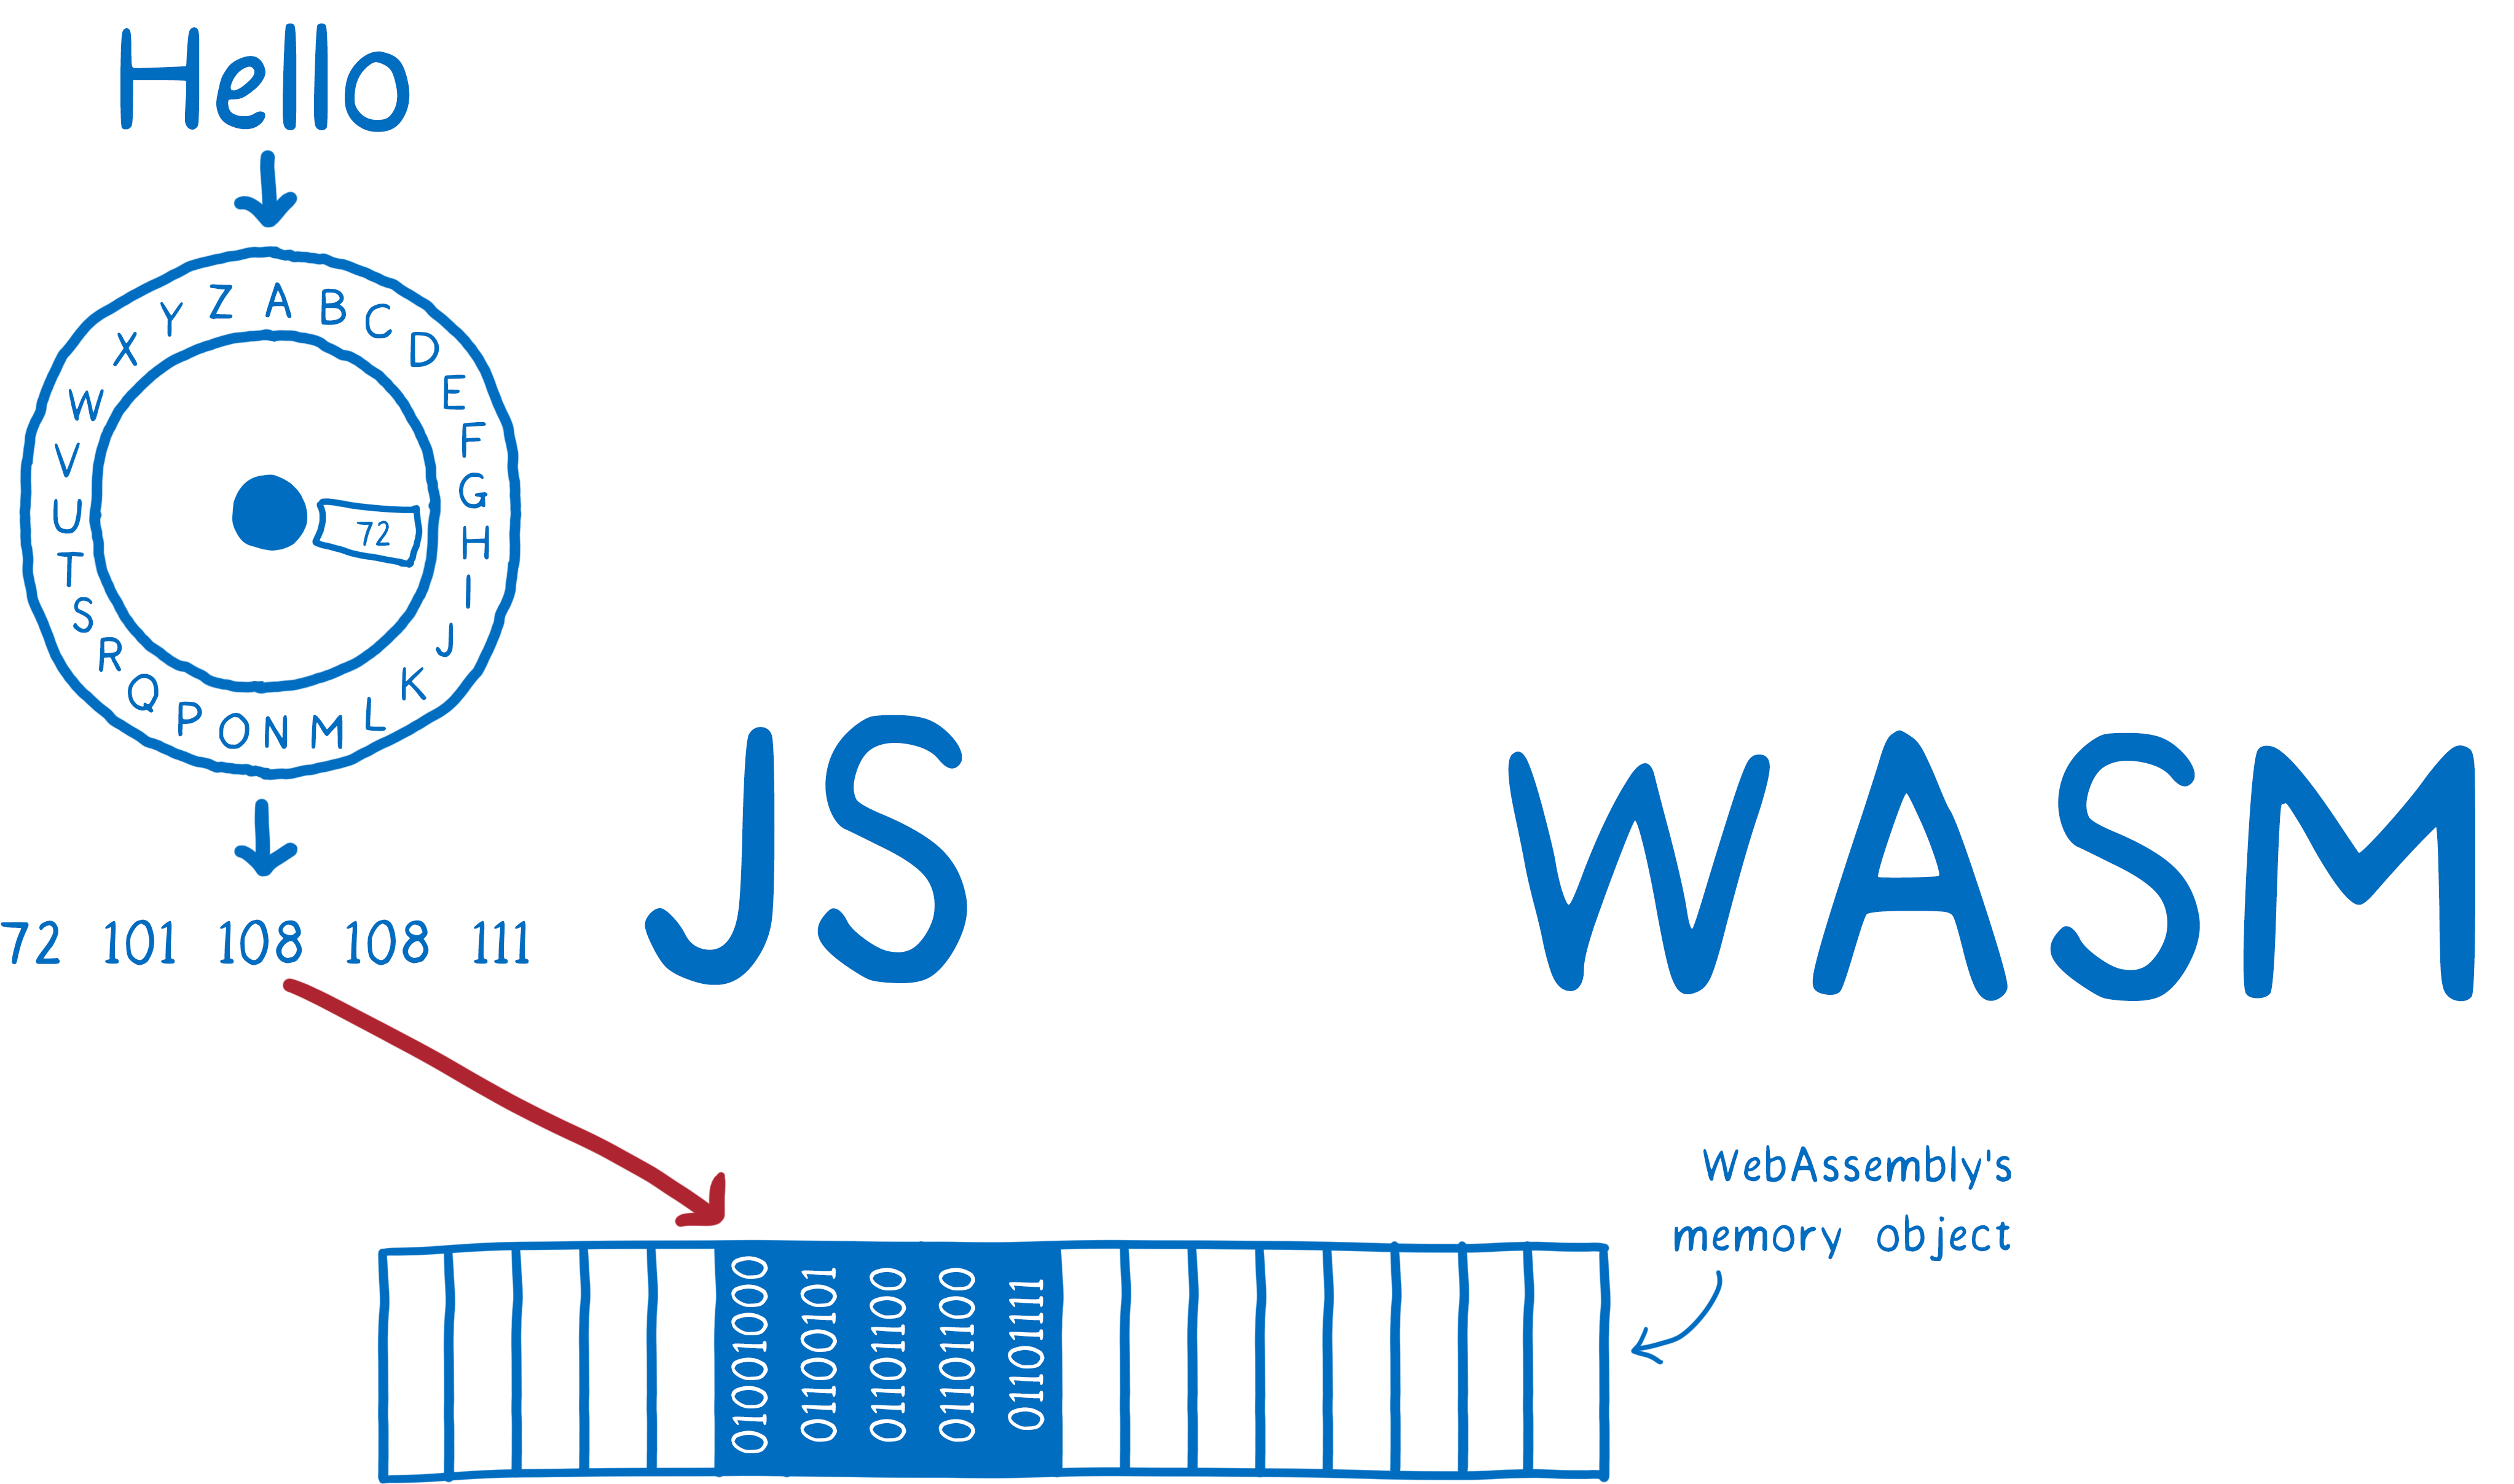
\includegraphics[width=\textwidth]{./figures/wasm_bindgen.png}

\clearpage

\section{Welke front- \& backend frameworks zijn er ter beschikking?}
\label{frameworks}

Om efficiënt webapplicaties te bouwen heb je natuurlijk een degelijk framework nodig die voor jou al
het zware werk doet. Gelukkig heeft Rust mits zijn jonge jaren, al een aardig aantal frameworks ter
beschikking voor het bouwen van webapplicaties.  

Dit zijn de top 3 front- en backend frameworks. Gerangschikt naar mate van hun populariteit (GitHub
stars).

\subsection{Frontend}

\subsubsection{Yew - 21k} 

Yew is het populairste frontend framework met over 21k GitHub stars. Het beschikt
over een component-gebaseerd framework dat het makkelijk maakt om interactieve UI’s te maken.
Ontwikkelaars die ervaring hebben met frameworks als React en Elm zouden zich helemaal thuis moeten
voelen bij het gebruik van Yew. Naast de aangename developer experience brengt het ook geweldige
prestaties met zich mee. Dit bereiken ze door het minimaliseren van het aanroepen naar de DOM en
door ontwikkelaars te helpen om gemakkelijk taken te offloaden naar achtergrond threads met behulp
van web workers. 

De documentatie over de huidige release versie 19.0 is uitgebreid geschreven.  Er kan zelfs al
gekeken worden naar de volgende release “Next”, die refereert naar de master branch. In de Next
versie is belangrijkste nieuwe feature SSR, want de huidige versie heeft alleen maar CSR.

\subsubsection{Dixous - 3.8k}

Dixous is een opkomend en jong UI framework als concurrent voor Yew. Het is net als Yew ontworpen om
React-achtig te zijn. Zo heeft het ook een component-gebaseerde architectuur, state management,
props en nog veel meer. Buiten de verschillende syntax tegen over Yew, heeft Dixous nog een aantal
troeven zoals:  
\begin{itemize}
  \item de keuze tussen JSX-achtige of hun eigen macro gebaseerde RSX syntax als templating systeem
    ingebouwde globale state en error handler 

  \item components en hooks kunnen worden hergebruikt voor te renderen op het web, desktop, mobiel,
    server en meer 

  \item uitgebreide inline documentatie 

  \item SSR 
\end{itemize}

\subsubsection{Seed - 3.3k}

Seed is een frontend framework voor het maken van prestatiegerichte en betrouwbare webapps die een
Elm-achtige architectuur heeft. Het heeft een minimale configuratie en boilerplate, en heeft
duidelijke documentatie die het voor iedereen gemakkelijk maakt om mee te beginnen.  

Ook Seed gebruikt een eigen templating systeem met een macro syntax waardoor Rustaceans zich meteen
thuis voelen. Dit betekent dat linting, formatteren en commentaar geven zullen werken, en het is
allemaal in Rust. Dit in tegenstelling tot een JSX-achtige syntax (zoals die van Yew) die
afhankelijk is van IDE-extensies om de developer experience te verbeteren. 

Seed beschikt niet over SSR en heeft nog geen plannen om het te implementeren. 

\subsection{Backend}

\subsubsection{Rocket – 17.2k}

Rocket is een populair webframework dat het voor developers gemakkelijk maakt om snelle webapps te
schrijven zonder te bezuinigen op veiligheid, flexibiliteit of functionaliteiten. Het heeft
ondersteuning voor het testen van libraries, cookies, streams, routes, templates, databases, ORMs,
boilerplates, en nog veel meer. Rocket heeft ook een grote en actieve community. 

\subsubsection{Actix-web – 14.1k}

Net als Rocket, is Actix een ander krachtig backend web framework. Actix heeft een
architectuurpatroon gebaseerd op het actor-systeem van Rust en is goed uitgerust voor het bouwen van
schrijfdiensten en micro apps. Het heeft ondersteuning voor routing, middleware, testen, WebSockets,
automatisch server reloading en kan gehost worden op NGINX. Actix kan worden gebruikt om een
volledige web app en API te bouwen. 

\subsubsection{Axum – 4.7k}

Alhoewel er nog populairdere frameworks zijn dan Axum verdient het zeker een plaats in de top 3.
Axum is deel van het populaire Tokio project, met sponsors als aws, azure en facebook. Tokio is een
asynchrone runtime voor Rust, die de bouwstenen biedt die nodig zijn voor het schrijven van
netwerktoepassingen. 

Axum is een laag bovenop Tokio’s HTTP client genaamd hyper, die een relatief low-level library is en
bedoeld is al bouwsteen voor libraries en applicaties. Het framework focust op ergonomie en
modulariteit. Wat het nog onderscheidt met andere frameworks, is dat het geen eigen middleware
systeem heeft maar gebruikt in plaats daarvan de tower::Service module van het Tokio project. Dit
betekent dat Axum gratis timeouts, tracing, compressie, authorisatie en meer krijgt. 

Dit alles maakt met zijn jonge 1-jarige leeftijd toch een library om naar uit te kijken. 

\clearpage

\section{Hoe bouw je een web app in Rust?}

Sinds Yew het populairste framework is en ook is gebruikt als framework voor het bouwen van de speed
typing applicatie, zal de vraag \enquote{Hoe bouw je een Webapplicatie in Rust} beantwoord worden met Yew
als framework. Het bouwen van een webapplicatie in een ander framework zal in grote lijnen hetzelfde
zijn. Dit zal een praktische kijk zijn op hoe we Yew kunnen gebruiken voor het bouwen van
Webapplicaties.  

In dit voorbeeld gaan we een simpele Todo applicatie bouwen.

\subsection{Tools installeren}

\subsubsection{Rust}
Om Rust te installeren hebben we de rustup toolchain installer nodig. Met het onderstaand script kan
je het installeren op jouw UNIX machine. Als je Rust al hebt staan maak dan zeker dat je de laatste
versie hebt door rustup update uit te voeren.

\begin{minted}{bash}
curl --proto '=https' --tlsv1.2 -sSf https://sh.rustup.rs | sh
\end{minted}

\subsubsection{WebAssembly}

Rust kan source codes compileren voor verschillende 'targets' (m.a.w verschillende processors). Het
compilatie target voor een browser gebaseerd WebAssembly heet wasm32-unkown-unkown. Het volgende
commando zal het WebAssembly target toevoegen aan je development environment.

\begin{minted}{bash}
rustup target add wasm32-unknown-unknown
\end{minted}

\clearpage

\subsubsection{Trunk}

De documentatie van Yew raad aan om Trunk te gebruiken voor het beheren van deployment en packaging.

\begin{minted}{bash}
cargo install --locked trunk
\end{minted}

Nu ons development enviroment opgezet is, kunnen we een nieuw cargo project aanmaken.

\begin{minted}{bash}
cargo new yew-app
cd yew-app
\end{minted}

Om te verifieren dat het Rust environment juist is opgezet, voer je het initiele project uit met de
cargo build tool. Na de output van de het build process, zou je normaal \mintinline{rust}{"Hello,
world!"} te zien
krijgen.

\begin{minted}{bash}
cargo run
\end{minted}

\subsubsection{Statische pagina}

Om deze simpele command line applicatie naar een basis Yew web applicatie te convertern, zijn er een
paar aanpassingen nodig. Pas de volgende bestanden aan als volgt:

\begin{listing}[h]
\begin{minted}{toml}
[package]
name = "yew-app"
version = "0.1.0"
edition = "2021"

[dependencies]
yew = "0.19"
\end{minted}
\caption{Cargo.toml}
\end{listing}

\clearpage

\begin{listing}[h]
\begin{minted}{rust}
use yew::prelude::*;

#[function_component(App)]
fn app() -> Html {
    html! {
        <h1>{ "Hello World" }</h1>
    }
}

fn main() {
    yew::start_app::<App>();
}
\end{minted}
\caption{main.rs}
\end{listing}

Maak nu een index.html aan in de root folder van het project.

\begin{listing}[h]
\begin{minted}{html}
<!DOCTYPE html>
<html lang="en">
  <head> </head>
  <body></body>
</html>
\end{minted}
\caption{index.html}
\end{listing}

\subsubsection{Start de development server}

Voer het volgende commando uit om de applicatie te builden en lokaal te draaien.

\begin{minted}{bash}
trunk serve --open
\end{minted}

\subsection{Statische pagina}

\subsubsection{Bouwen van HTML}

Yew maakt gebruik van de procedurele macro's van Rust en biedt ons een syntax die lijkt op JSX (een
uitbreiding van JavaScript waarmee u HTML-achtige code kunt schrijven in JavaScript) om de opmaak te
maken.

\clearpage

\subsubsection{Converteren van HTML naar Rust}

Aangezien we al een vrij goed idee hebben van hoe onze website eruit zal zien, kunnen we onze
mentale opzet eenvoudig vertalen naar een voorstelling die compatibel is met html!. Als je
eenvoudige HTML kunt schrijven, moet het geen probleem zijn om markeringen in html! te schrijven.
Het is belangrijk op te merken dat de macro op een paar punten verschilt van HTML:
\begin{itemize}
  \item Uitdrukkingen moeten tussen accolades staan (\{ \})
  \item Er mag maar één root node zijn. Als je
    meerdere elementen wilt hebben zonder ze in een container te wikkelen, wordt een lege
    tag/fragment (<> ... </>) gebruikt
  \item Elementen moeten goed worden afgesloten.
\end{itemize}

We willen een layout bouwen die er ongeveer zo uitziet in ruwe HTML:

\begin{minted}{html}
<main>
  <h1>My todo list</h1>
  <ul>
    <li>
      <input type="checkbox" />
      <label>Take dog out for a walk</label>
    </li>
    <input type="checkbox" />
    <label>Feed the cats</label>
    <li>
      <input type="checkbox" />
      <label>Take out the trash</label>
    </li>
    <li>
      <input type="checkbox" />
      <label>Water plants</label>
    </li>
  </ul>
</main>
\end{minted}

\clearpage

Laten we nu deze HTML in html! omzetten. Type (of kopieer/plak) het volgende knipsel in de body van
de app functie, zodat de waarde van html! wordt geretourneerd door de functie.

\begin{listing}[h]
\begin{minted}{rust}
#[function_component]
pub fn App() -> Html {
  html! {
    <main>
      <h1>{ "My todo list" }</h1>
      <ul>
        <li>
          <input type="checkbox"/>
          <label> { "Take dog out for a walk" } </label>
        </li>
          <input type="checkbox"/>
          <label> { "Feed the cats" } </label>
        <li>
          <input type="checkbox"/>
          <label> { "Take out the trash" } </label>
        </li>
        <li>
          <input type="checkbox"/>
          <label> { "Water plants" } </label>
        </li>
      </ul>
    </main>
  }
}
\end{minted}
\caption{app.rs}
\end{listing}

\clearpage

\subsubsection{Components}

Components zijn de bouwstenen van Yew applicaties. Door components te combineren, die weer uit
andere components kunnen worden opgebouwd, bouwen we onze applicatie. Door onze components te
structureren voor herbruikbaarheid en ze generiek te houden, kunnen we ze in meerdere delen van onze
applicatie gebruiken zonder code of logica te hoeven dupliceren.

In feite is de app functie die we tot nu toe hebben gebruikt een component, genaamd
\mintinline{rust}{App}. Het is een 'function component'. Er zijn twee verschillende soorten
componenten in Yew:
\begin{itemize}
  \item Struct Components 
  \item Function Components
\end{itemize}

In dit voorbeeld zullen we function components gebruiken.

Laten we nu onze \mintinline{rust}{App} component opsplitsen in kleinere componenten. We kunnen onze
Todo lijst opspliten in 2 components genaamd \mintinline{rust}{Task} en \mintinline{rust}{TaskList}.

\begin{listing}[h]
\begin{minted}{rust}
#[derive(Properties, Debug, PartialEq)]
pub struct TaskProps {
  pub id: String,
  pub title: String,
  pub completed: bool,
}

#[function_component]
pub fn Task(
  TaskProps {
    id,
    title,
    completed,
  }: &TaskProps,
) -> Html {
  html! {
    <li>
      <input
        type="checkbox"
        id={id.clone()}
        checked={*completed}
      />
      <label
        for={id.clone()}>{title.clone()}
      </label>
    </li>
  }
}
\end{minted}
\caption{task.rs}
\end{listing}

\clearpage

Let op de parameters van onze \mintinline{rust}{Task} function component. Een function component
heeft slechts één argument dat zijn 'props' (kort voor 'properties') definieert. Props worden
gebruikt om gegevens door te geven van een ouder component naar een kind component. In dit geval is
\mintinline{rust}{TaskProps} een \mintinline{rust}{struct} die de props definieert.

\begin{listing}[h]
\begin{minted}{rust}
#[derive(Properties, PartialEq)]
pub struct TaskListProps {
  pub children: Children,
}
#[function_component]
pub fn TaskList(TaskListProps { children }: &TaskListProps) -> Html {
  html! {
    <ul>
      { for children.iter() }
    </ul>
  }
}
\end{minted}
\caption{task\_list.rs}
\end{listing}

Nu kunnen we onze \mintinline{rust}{App} component updaten met onze nieuwe components
\mintinline{rust}{Task} \& \mintinline{rust}{TaskList}.

\begin{listing}[h]
\begin{minted}{rust}
#[function_component]
pub fn App() -> Html {
  let tasks = vec![
    html! { 
      <Task id={"1"} title={"Take dog out for a walk"} completed={true} /> 
    },
    // ... andere tasks
  ];
  html! {
    <main>
      <h1>{ "My todo list" }</h1>
      <TaskList>
        {tasks}
      </TaskList>
    </main>
  }
}
\end{minted}
\caption{app.rs}
\end{listing}

\clearpage

\subsubsection{Interactief}
Momenteel doet onze applicatie niet veel anders dan onze voor gedefineerde lijst te tonen.
Uiteindlijk willen we onze taken uit de todo lijst kunnen schrappen. Om deze interactie te laten
werken zullen we een aantal zaken aanpassen.

Om bij te houden of de gebruiker de taak geschrapt heeft al dan niet, zullen we een
\mintinline{rust}{completed_state} gebruiken met de \mintinline{rust}{use_state} hook. Zo verliezen
we niet de waarde van de variabele \mintinline{rust}{completed_state} mocht het component
re-renderen.

\begin{minted}{rust}
#[function_component]
pub fn Task(
    ...
) -> Html {
    let completed_state = use_state(|| *completed);
    ...
}
\end{minted}

Het volgende is natuurlijk het \mintinline{rust}{onclick} event afhandelen als de gebruiker op het
label of input element klikt. Hiervoor hebben we een \mintinline{rust}{Callback} functie nodig die
onze \mintinline{rust}{completed_state} aanpast naargelang de vorige state. Voor we de
\mintinline{rust}{completed_state} kunnen gebruiken in onze Callback closure functie moeten we die
eerst clonen. De reden hiervoor is het keyword \mintinline{rust}{move} die voor de closure
parameters staat, \mintinline{rust}{move} zorgt
ervoor dat alle references die gebruikt worden in de closure scope hun waarden worden verplaatst
binnen de scope. Dus om te voorkomen dat we onze \mintinline{rust}{completed_state} nergens meer
kunenn gebruiken clonen we eerst de state.

Daarnaast kunnen we ook een css class meegeven met de \mintinline{rust}{classes!} macro van yew, die
conditioneel het html label zal doorstrepen al dan niet.

\clearpage

\begin{listing}
\begin{minted}{rust}
#[function_component]
pub fn Task(
    TaskProps {
        id,
        title,
        completed,
    }: &TaskProps,
) -> Html {
    let completed_state = use_state(|| *completed);

    let onclick = {
        let completed_state = completed_state.clone();

        Callback::from(move |_| {
            if *completed_state {
                completed_state.set(false);
            } else {
                completed_state.set(true);
            }
        })
    };

    let completed_class = {
        if *completed_state {
            "line-through"
        } else {
            ""
        }
    };

    html! {
        <li>
            <input
                {onclick}
                type="checkbox"
                id={id.clone()}
                checked={*completed_state}
            />
            <label
                class={classes!(completed_class)}
                for={id.clone()}>{title.clone()}
            </label>
        </li>
    }
}
\end{minted}
\caption{task.rs}
\end{listing}

\clearpage

\subsubsection{Data extern ophalen}

In de speed typing applicatie komen de code snippets van een API in plaats van hard gecodeerd te
zijn in de frontend. Laten we onze todo lijst ophalen van een externe bron. Hiervoor moeten we de
volgende crates toevoegen:
\begin{itemize}
  \item reqwasm voor het maken van de fetch call.
  \item serde met derive functies Voor het de-serialiseren van het JSON antwoord
  \item wasm-bindgen-futures voor het uitvoeren van Rust Future als een Promise
\end{itemize}

Laten we de dependencies in het Cargo.toml bestand bijwerken:

\begin{minted}{toml}
[dependencies]
yew = { git = "https://github.com/yewstack/yew/", features = ["csr"] }
serde = { version = "1.0", features = ["derive"] }
wasm-bindgen-futures = "0.4"
\end{minted}

Pas de \mintinline{rust}{TaskProps} struct aan om de \mintinline{rust}{Deserialize} trait af te leiden.

\begin{minted}{rust}
#[derive(Properties, Debug, PartialEq, Deserialize)]
pub struct TaskProps {
  pub id: String,
  pub title: String,
  pub completed: bool,
}
\end{minted}

Als laatste stap moeten we onze App component updaten om de fetch request te maken in plaats van
hardcoded data te gebruiken.

Hier gebruiken we de \mintinline{rust}{use_effect_with_deps} hook met lege dependencies als tweede
parameter om de tasks slechts eenmaal op te halen bij de eerste render van het App component. In de
closure gebruiken we \mintinline{rust}{wasm-bindgen-futures} om de Javascript Promise die de
\mintinline{rust}{Request::get} genereert om te zetten naar een Future type. Met de
\mintinline{rust}{Request::get} halen we de JSON todos op en slaan ze op als een
\mintinline{rust}{vec} met \mintinline{rust}{TaskProps}. Vervolgens vullen we onze
\mintinline{rust}{tasks} state met de \mintinline{rust}{fetched_tasks} en zullen de tasks worden
weergeven in de browser!

\begin{listing}
\begin{minted}{rust}
#[function_component]
pub fn App() -> Html {
let tasks = use_state(std::vec::Vec::new);
  {
    let tasks = tasks.clone();
    use_effect_with_deps(move |_| {
      wasm_bindgen_futures::spawn_local(async move {
        let fetched_tasks: Vec<TaskProps> = Request::get("url")
          .send()
          .await
          .unwrap()
          .json()
          .await
          .unwrap();

        tasks.set(fetched_tasks.iter().take(10).map(|props| {
            html! { 
              <Task 
                id={props.id.clone()} 
                title={props.title.clone()} 
                completed={props.completed} 
              /> 
            }
          }).collect()
        );
      });
      || ()
    }, ());
  }

  html! {
      <main>
          <h1>{ "My todo list" }</h1>
          <TaskList>
              { (*tasks).clone() }
          </TaskList>
      </main>
  }
}
\end{minted}
\caption{app.rs}
\end{listing}

\clearpage

\section{Hoe bouw je een API in Rust?}

Volgend op de Todo applicatie die we gebouwd hebben in "Hoe bouw je een web app in Rust?",
zullen we een REST API bouwen die de taken uit een database zal halen en opslaan. Als API framework
zullen we Actix-web gebruiken, samen met diesel.rs als ORM voor het beheren van de database. Om het
simpel te houden gebruiken we net zoals in de speed typing test applicatie SQLite als database.


\subsection{Opzet project}

Maak een nieuw Rust project aan met de volgende dependencies.

\begin{minted}{bash}
cargo new api
cd api/
\end{minted}

\begin{listing}[h]
\begin{minted}{toml}
[dependencies]
diesel = { version = "1.4.8", features = ["sqlite", "r2d2"] }
dotenv = "0.15.0"
actix-web = "4"
actix-cors = "0.6.1"
uuid = { version = "0.8", features = ["serde", "v4"] }
serde = { version = "1.0", features = ["derive"] }
serde_json = "1.0"
log = "0.4"
env_logger = "0.9.0"
\end{minted}
\caption{Cargo.toml}
\end{listing}

We zullen uitleggen waarom we deze dependencies nodig hebben als we verder gaan.

\subsubsection{Database}

Diesel biedt een aparte CLI tool om je project te helpen beheren. Omdat het een standalone binary
is, en geen directe invloed heeft op de code van je project, voegen we het niet toe aan Cargo.toml.
In plaats daarvan installeren we het gewoon op ons systeem.

\begin{minted}{bash}
echo DATABASE_URL=todo.db > .env
\end{minted}

Nu kan Diesel CLI alles voor ons opzetten.

\begin{minted}{bash}
diesel setup
\end{minted}

Dit zal onze database aanmaken (als die nog niet bestond), en een lege migrations directory aanmaken
die we kunnen gebruiken om ons schema te beheren.

Diesel support momenteel alleen een database-first aanpak. Hierbij maken we eerst het database
schema om dan met migrations het schema naar Rust om te zetten. Dat gezegd zijnde, laat ons een
eerste migration aanmaken.

\begin{minted}{bash}
diesel migration generate create_tasks
\end{minted}

Diesel CLI zal twee lege bestanden (\mintinline{rust}{up.sql} en \mintinline{rust}{down.sql}) voor
ons aanmaken in de vereiste structuur. In deze bestanden schrijven we SQL voor de Task tabel aan te
maken in \mintinline{rust}{up.sql} en als we de migration willen ongedaan maken in
\mintinline{rust}{down.sql}.

\begin{listing}
\begin{minted}{sql}
CREATE TABLE tasks (
  id VARCHAR NOT NULL PRIMARY KEY,
  title VARCHAR NOT NULL,
  completed INTEGER NOT NULL DEFAULT 0
)
\end{minted}
\caption{up.sql}
\end{listing}

\begin{listing}
\begin{minted}{sql}
DROP TABLE tasks
\end{minted}
\caption{down.sql}
\end{listing}

Nu kunnen we onze eerste migration uitvoeren met:

\begin{minted}{bash}
diesel migration run
\end{minted}

Dit zal onze SQL migration uitvoeren op de \mintinline{bash}{todo.db} database en het nodige Rust
schema genereren met de nodige types. In het Rust schema wordt met de \mintinline{rust}{table!}
macro een hoop code gegeneerd gebaseerd op het database schema om alle tabellen en kolommen weer te
geven. Zo kunnen we nu gebruik maken van Rust zijn krachtig typesysteem om volledige SQL queries te
gaan bouwen met code. We zullen in het volgende voorbeeld zien hoe we dat precies kunnen gebruiken.

Telkens wanneer we een migratie uitvoeren of terugdraaien, wordt dit bestand automatisch bijgewerkt.

\clearpage

\subsection{API}

Om de basis functionaliteiten van onze Todo applicatie in de front-end te ondersteunen, zal onze API
een nieuwe taak kunnen aanmaken en de lijst met taken ophalen. Dus zullen we de volgende endpoints
hebben:
\begin{itemize}
  \item GET /tasks - retourneert alle taken
  \item POST /tasks - voegt een nieuwe taak toe
\end{itemize}


Om onze code overzichtelijklijk te houden, zullen we de volgende structuur hanteren:
\dirtree{%
.1 src/.
.2 main.rs.
.2 models.rs.
.2 schema.rs.
.2 handlers.rs.
.2 db.rs.
}

Bij het opzetten van ons project heeft cargo een al een \mintinline{bash}{main.rs} bestand
aangemaakt. Laten we dat bewerken en onze eerste \mintinline{rust}{"Hello World!"} route schrijven.

\begin{listing}[h]
\begin{minted}{rust}
use actix_web::{web, App, HttpServer};

#[actix_web::main]
async fn main() -> std::io::Result<()> {
  HttpServer::new(|| {
    App::new()
      .route("/hello", web::get().to(|| async { "Hello World!" }))
  })
  .bind(("127.0.0.1", 5000))?
  .run()
  .await
}
\end{minted}
\caption{main.rs}
\end{listing}
\clearpage

Onze main functie heeft nu het \mintinline{rust}{#[actix_web::main]} attribuut, die zal onze main
functie markeren als start functie en uitvoeren in de runtime van \mintinline{rust}{actix_web}.

Een belangrijk punt om op te merken is dat we een \mintinline{rust}{Result} type teruggeven. Dit
stelt ons in staat om de \mintinline{rust}{?} operator in main te gebruiken, die elke fout die door
de geassocieerde functie wordt teruggegeven naar de aanroeper koppelt.

Het tweede ding om op te merken is \mintinline{rust}{async/await}. Hiermee geven we aan dat Rust
onze functies asynchroon kan uitvoeren zonder andere threads te blokkeren.

In onze main, instantiëren we een \mintinline{rust}{HttpServer}, voegen er een
\mintinline{rust}{App} aan toe die dient als een
Application factory en voegen onze eerste route er aan toe.

Als alles goed gaat zou je nu de API kunnen opstarten met \mintinline{bash}{cargo run} en bij een
GET request naar \mintinline{bash}{localhost:8080/hello} \mintinline{rust}{"Hello world!"} als repons 
te zien krijgen.

\begin{listing}[h]
\begin{minted}{rust}
#[get("/task")]
async fn get_tasks() -> Result<HttpResponse, Error> {
  todo!()
}

#[post("/task")]
async fn add_task() -> Result<HttpResponse, Error> {
  todo!()
}
\end{minted}
\caption{handlers.rs}
\end{listing}

In de module \mintinline{rust}{handlers} zullen we onze requests per endpoint afhandelen. Voorlopig
gebruiken we hier nog de \mintinline{rust}{todo}! macro sinds we nog geen communicatie maken de
database. Laat ons dat eerst aanpakken.

Onze eerste migration die we eerder hebben uitgevoerd heeft voor ons al een
\mintinline{rust}{schema.rs} module aangemaakt, zodat diesel onze queries kan controleren tijdens
het compileren. Om met queries te kunnen werken in Rust hebben we models nodig. Zo kunnen we het
resultaat van een query mappen naar een model of een model gebruiken voor nieuwe data in te voegen.

Met de traits \mintinline{rust}{Queryable} en \mintinline{rust}{Insertable} zorgen we er voor dat de
struct \mintinline{rust}{Task} als resultaat voor een query kan gebruikt worden en als struct om
nieuwe data in te voegen.

\mintinline{rust}{Deserialize} en \mintinline{rust}{Serialize} komen van de crate
\mintinline{rust}{serde}, zij zorgen ervoor dat we de models kunnen omzetten naar json en andersom.

\clearpage

\begin{listing}[h]
\begin{minted}{rust}
#[derive(Debug, Serialize, Deserialize, Queryable, Insertable)]
pub struct Task {
  pub id: String,
  pub title: String,
  pub completed: bool,
}

#[derive(Debug, Serialize, Deserialize)]
pub struct InputTask {
  pub title: String,
}
\end{minted}
\caption{models.rs}
\end{listing}

Nu we onze models hebben kunnen we in \mintinline{rust}{db} functies schrijven om tasks op te vragen
en aan te maken. De functies spreken voorzich, we gebruiken diesel zijn sql implementaties om met
onze database te communiceren.

Merk op dat we bij elke functie \mintinline{rust}{schema::tasks::dsl::*} opnieuw toevoegen aan de
lokale scope. Dit is puur conventie sinds we maar 1 tabel hebben \mintinline{rust}{Tasks}, moesten
we meerdere tabellen hebben zouden we onze scope kunnen vervuilen door bijvoorbeeld zelfde
kolomnamen die elkaar overschrijven.

\begin{listing}[h]
\begin{minted}{rust}
type DbError = Box<dyn std::error::Error + Send + Sync>;

pub fn list_all_tasks(conn: &SqliteConnection) 
  -> Result<Option<Vec<Task>>, DbError> {
  use crate::schema::tasks::dsl::*;
  Ok(tasks.load::<Task>(conn).optional()?)
}
pub fn insert_new_task(t: &str, conn: &SqliteConnection) 
  -> Result<Task, DbError> {
  use crate::schema::tasks::dsl::*;
  let new_task = Task {
    id: Uuid::new_v4().to_string(),
    title: t.to_owned(),
    completed: false,
  };
  diesel::insert_into(tasks).values(&new_task).execute(conn)?;
  Ok(new_task)
}
\end{minted}
\caption{db.rs}
\end{listing}

\clearpage

Nu we onze helper functies geschreven hebben kunnen we de requests afhandelen in
\mintinline{rust}{handlers} als volgt:

Elke handler functie krijgt een connection pool als parameter, die we later zullen definieren in
main. De connection pool zal verschillende connecties met de database openhouden zodat ze efficient
kunnen hergebruikt worden door anderen. Om te voorkomen dat een andere thread de connectie gebruikt
tijdens het uitvoeren van een \mintinline{rust}{db} functie blokkeren we deze thread met
\mintinline{rust}{web::block}. Als alles goed verloopt geven we de resultaten terug, indien niet
geven we een \mintinline{rust}{InternalServerError} terug.

\begin{listing}[h]
\begin{minted}{rust}
#[get("/task")]
async fn get_tasks(
  pool: web::Data<DbPool>,
) -> Result<HttpResponse, Error> {
  let tasks = web::block(move || {
    let conn = pool.get()?;
    db::list_all_tasks(&conn)
  })
  .await?
  .map_err(actix_web::error::ErrorInternalServerError)?;

  if let Some(tasks) = tasks {
    Ok(HttpResponse::Ok().json(tasks))
  } else {
    let res = HttpResponse::NotFound().body("No tasks found!".to_string());
    Ok(res)
  }
}
#[post("/task")]
async fn add_task(
  pool: web::Data<DbPool>,
  form: web::Json<models::InputTask>,
) -> Result<HttpResponse, Error> {
  let task = web::block(move || {
    let conn = pool.get()?;
    db::insert_new_task(&form.title, &conn)
  })
  .await?
  .map_err(actix_web::error::ErrorInternalServerError)?;

  Ok(HttpResponse::Created().json(task))
}
\end{minted}
\caption{handler.rs}
\end{listing}

\clearpage

Wat ons nu nog rest te doen, is onze connection pool instantiëren en de handler functies linken aan
onze App. Vooraleer dat we dat doen laden we eerst ons .env bestand in het enviroment met de
\mintinline{rust}{dotenv} crate en loggen we info over de applicatie naar \mintinline{bash}{stdout}
met \mintinline{rust}{env_logger}. Daarna kunnen we onze connection pool opzetten met de
\mintinline{bash}{DATABASE_URL} uit het enviroment. Ten slotte voegen we onze hanlder functies toe
aan een nieuwe service met als scope \mintinline{bash}{/api} zodat al onze routes worden ge prefixed
met \mintinline{bash}{/api}.

\begin{listing}[h]
\begin{minted}{rust}
type DbPool = r2d2::Pool<ConnectionManager<SqliteConnection>>;
#[actix_web::main]
async fn main() -> std::io::Result<()> {
  dotenv::dotenv().ok();
  env_logger::init_from_env(
    env_logger::Env::new().default_filter_or("info")
  );
  // set up database connection pool
  let conn_spec = std::env::var("DATABASE_URL").expect("DATABASE_URL");
  let manager = ConnectionManager::<SqliteConnection>::new(conn_spec);
  let pool = r2d2::Pool::builder()
    .build(manager)
    .expect("Failed to create pool.");
  log::info!(
    "{}",
    format!("starting HTTP server at http://localhost:5000"
  ));
  // Start HTTP server
  HttpServer::new(move || {
    App::new()
      .app_data(web::Data::new(pool.clone()))
      .wrap(middleware::Logger::default())
      .service(
        web::scope("/api")
        .service(get_tasks)
        .service(add_task)
      )
    })
  .bind(("127.0.0.1", 5000))?
  .run()
  .await
}
\end{minted}
\caption{main.rs}
\end{listing}


\clearpage

\section{Is Rust productie klaar?}
\label{productie}

Wanneer een taal 'productie klaar' benoemd kan worden is eigenlijk een moeilijke vraag om te
beantwoorden. Wat 'productie klaar' betekent hangt af van verschillende factoren voor een specifiek
domein. Rust schittert bijvoorbeeld in productief veilige en performante applicaties te bouwen. Top
bedrijven zoals Amazon, Facebook, Microsoft kunnen dit beamen sinds ze ondertussen al een aantal jaar
Rust gebruiken \cite{rust_companies}. Zo heeft Amazon in 2018 Firecracker gelanceerd
\cite{aws_sustainability}. Een open source virtualisatietechnologie die AWS Lambda en andere
serverloze aanbiedingen aandrijft. Daarnaast gebruiken ze Rust ook voor services te leveren zoals
Amazon Simple Storage Service (Amazon S3), Amazon Elastic Compute Cloud (Amazon EC2), Amazon
CloudFront, en meer. Amazon heeft dan ook samen met Google, Microsoft, Huawei en Mozilla de Rust
foundation opgericht in 2020, met een missie om het developen van Rust te ondersteunen. We kunnen
dus concluderen dat de taal op zich wel een stabiele omgeving is. Dit onderzoek gaat natuurlijk wel
over hoe we Rust kunnen gebruiken voor het bouwen van webapplicaties. We richten onze focus dan ook
op dit domein. We zullen de deelvraag “Is Rust productie klaar?” opsplitsen in twee delen namelijk
frontend en backend. 

\subsection{Backend }

Laten we beginnen met de backend. Bij het bouwen van hedendaagse webapplicaties heb je over het
algemeen 2 zaken nodig, een API en een database. Uiteraard is dit niet altijd het geval maar laten
we onze focus hierop leggen. 

Om een web API te bouwen gebruik je gewoonlijk een web framework. Het huidige rust ecosysteem heeft
een aantal stabiele web frameworks ter beschikking. Uit de deelvraag “Hoe bouw je een API in
Rust?” hebben we gekozen voor Actix-web te gebruiken als framework. Actix-web voorziet alles wat je
kan verwachten van een web framework, van routing en middleware, tot templating en JSON/form
afhandeling. Het is ook een van de snelste web frameworks ter beschikking. Zo staat actix momenteel
op de 5de plaats bij een benchmark ranking van alle populaire web frameworks (ook andere
programmeertalen dan Rust) \cite{web_bench}. 

Het actix framework ondersteunt verschillende soorten databases zoals mongodb, postgres, redis,
sqlite, graphql, elasticsearch en meer. De ene database heeft meer ondersteuning dan de andere, maar
naarmate de tijd vordert zal de ondersteuning alleen maar verbeteren. 

\subsection{Frontend}

Bij de frontend komt er wat meer bij kijken. Er zijn namelijk twee opties waarvoor Rust gebruikt kan
worden: 
\begin{itemize}
  \item Een gedeelde in Rust schrijven en compileren naar wasm om vervolgens te importeren als een node
    module in een bestaande Javascript applicatie. 
  \item Een volledige frontend in Rust schrijven met een web framework als Yew en compileren naar wasm 
\end{itemize}               

\clearpage

De eerste optie is meteen ook de optie waarvoor wasm het meest zal gebruikt worden. Zo kan je
bijvoorbeeld Javascript gebruiken voor de UI en wasm voor de logica van de applicatie. Om mogelijks
meer performatie te winnen en correctere code te schrijven. Deze optie wordt al volop in productie
gebruikt door meerdere bedrijven \cite{made_with_wasm}: 
\begin{itemize}
  \item 1Password – gebruikt wasm om hun browser plugin te versnellen 
  \item Figma – gebruikt wasm om hun originele C++ applicatie te exporteren naar de browser 
  \item SketchUp – gebruikt wasm om een 3d modelling tool op het web te draaien, wat snelle en
    voorspelbare prestaties verreist 
\end{itemize}

De andere optie, een volledige frontend bouwen met Rust, is een optie die momenteel meer gebruikt
wordt voor hobby projecten dan voor productie. Een van de redenen hiervoor is dat het ecosysteem nog
zeer jong is. Het is bijvoorbeeld niet te vergelijken met het ecosysteem van populaire JS
frameworks, wat ook logisch is. Desondanks het ecosysteem wordt Yew aan een snel tempo ontwikkeld.
Waar sommige libraries als React jaren over doen om features uit te brengen als SSR doet Yew in elke
maanden.

Het is ook merkwaardig dat Yew degelijk scoort op benchmarks. Natuurlijk presteert Yew beter dan
Javascript frameworks in het werken met geheugen, maar wat vooral opvalt is dat het ook redelijk
presteert in het aanpassen van de DOM. Dit is nu nog een struikel punt voor WebAssembly in het
algemeen, sinds er nog altijd javascript functies worden gebruikt voor het aanpassen van de DOM.
Dat is een van de redenen waarom we hogere bundel grootes over het netwerk zien bij Yew.
Een andere reden is dat WebAssembly zelf niet beschikt over geheugen beheer en garbage collectors.
Om die reden wordt vaak een runtime meegeleverd met de logica van je applicatie. In sommige gevallen
(Rust) is deze runtime vrij licht, en in andere (Blazor) is het zeer zwaar. We zullen waarschijnlijk
zien dat het gewicht van deze runtimes in de loop van de tijd aanzienlijk zal afnemen door nieuwe
WebAssembly mogelijkheden (garbage collection, module caching) en betere compilatietechnieken
(ahead-of-time compilation).

De resultaten van de benchmakrs zijn terug te vinden in Bijlage \ref{appendix:bench}.

\subsection{Conclusie}

Om Rust in productie te gebruiken kan dus zeker. De vraag is alleen of dit enige meerwaarden heeft
voor het bedrijf. Het antwoord hierop is terug te vinden Hoofdstuk \ref{reflectie} reflectie waar
de vraag wordt afgetoetst met mensen uit de praktijk.

\chapter{Technisch onderzoek}

\section{Voorbereiding}

Het technisch onderzoek startte bij het lezen van “The book” een boek over de taal Rust geschreven
door Steve Klabnik, Carol Nichols en met contributies van de Rust community. Tijdens het lezen waren
er kleine code voorbeelden die u kon mee volgen. Dit maakte het makkelijker om de geavanceerde
hoofdstukken goed te begrijpen. 

Na een paar hoofdstukken diep in het boek was het tijd om de geleerde zaken tot de test te brengen.
De opdracht was om de miniversie van het gekende Linux commando grep te maken. Zo werd de geleerde
kennis over structs, ownership, enums en pattern matching, error handling, lifetimes en tests
praktisch toegepast.  

Op het einde van het boek was er een finaal project dat ook de laatste hoofdstukken bevatte. Het
project was het bouwen van een “simpele” multi-threaded server. Daar lag de focus op het werken met
meerdere threads, wat niet voor de hand ligt als u rekening moet houden met het geheugen. 

Na de taal onder de knie te hebben, werd er onderzoek gedaan naar WebAssembly. Mits het nog een
piepjonge technologie is, was er al heel wat documentatie/artikelen over te vinden op het web. Zo
begon het onderzoek bij de documentatie van Mozilla. Daar is alles te vinden om van start te gaan
met WebAssembly. Er zijn ook doorverwijzingen naar hun uitstekende geschreven blogposts die dieper
gaan op hoe WebAssembly precies werkt.

Vervolgens moest er een keuze gemaakt worden welke frameworks we zullen gebruiken voor het bouwen
van de webapplicatie. Na wat onderzoek dat beschreven staat in “Welke front- end backend frameworks
zijn er ter beschikking?”, is er gekozen voor Yew als frontend en Actix web samen met diesel.rs als
backend frameworks.

\clearpage

\section{Omschrijving}

Om de huidige status van Rust voor het bouwen van webapplicaties te onderzoeken, werd er gekozen
voor een speed typing test applicatie te maken.

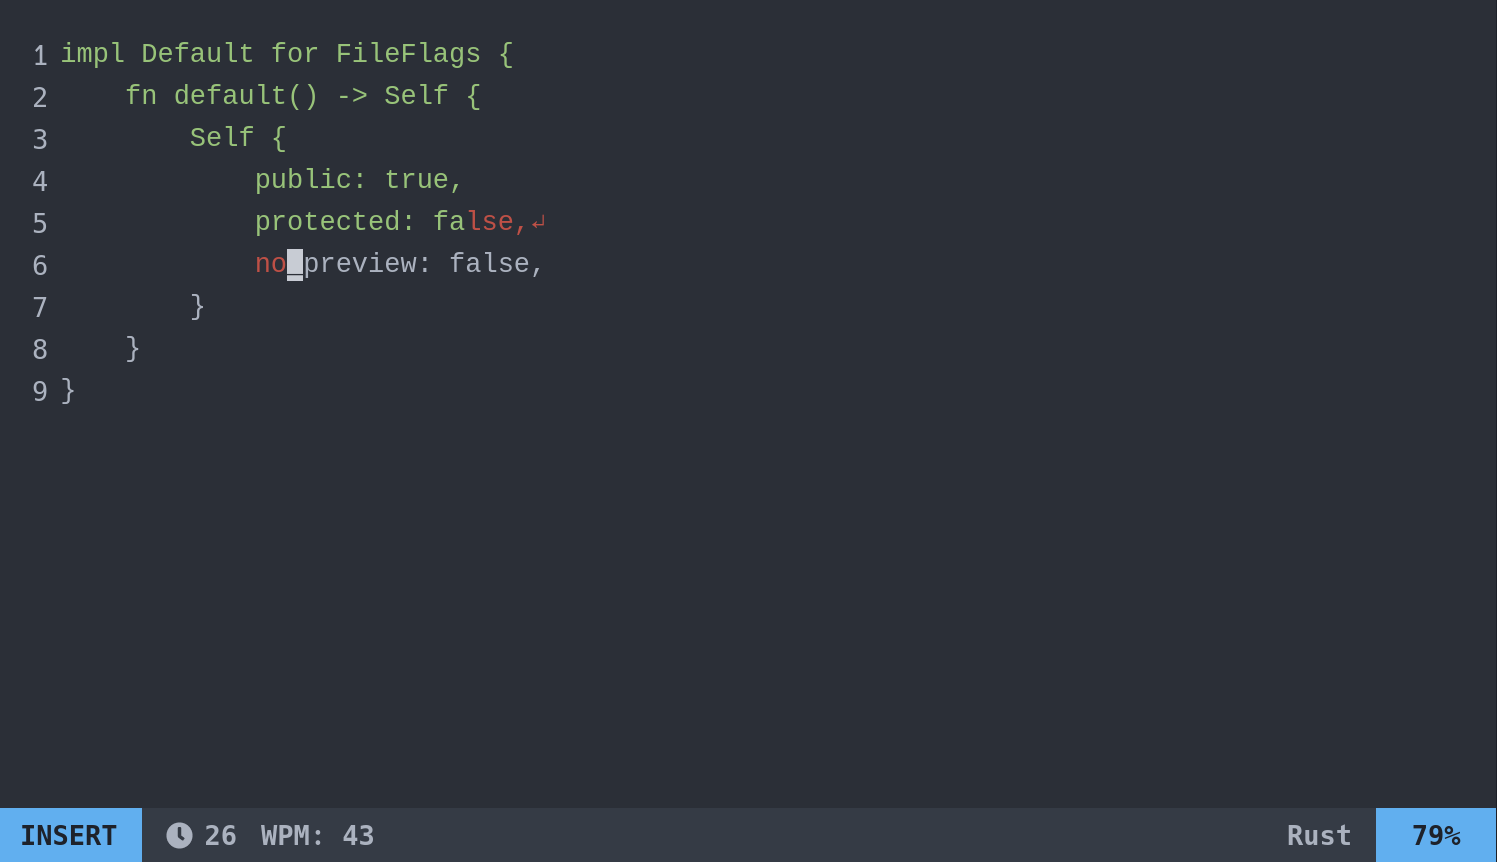
\includegraphics[width=\textwidth]{./figures/vim.png}

Het is een simpele applicatie waarbij de gebruiker een willekeurig code fragment krijgt die hij zo
snel mogelijk moet overtypen. Tijdens het typen wordt er live, zijn tijd en woorden per minut (WPM)
bijgehouden. Als de gebruiker het volledige fragment heeft overgetypt krijgt hij een resultaten
pagina te zien. Daar kan hij zijn statistieken bekijken zoals: WPM, verlopen tijd, accuraatheid en
het aantal fouten. Daarna kan de gebruiker opnieuw spelen door op de letter ‘r’ in te drukken. \\
\begin{wrapfigure}{l}{0.5\linewidth}
  \centering
  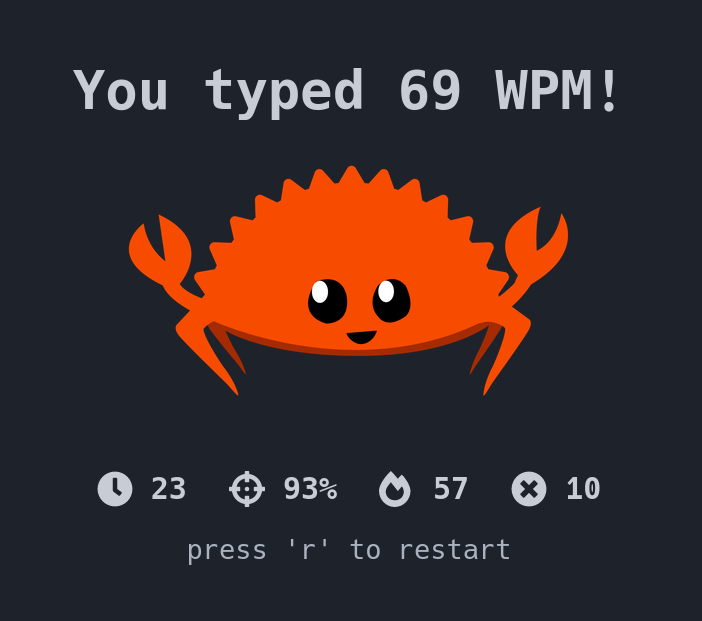
\includegraphics[width=0.9\linewidth]{./figures/result.png}
\end{wrapfigure}


Er was voor ogen om bij dit project nog een aantal functionaliteiten eraan toe te voegen. Zoals
authenticatie met SSO, de statistieken opslaan in de database zodat er een lijn grafiek kon getoond
op basis van de historiek, andere database, profiel pagina, ci/cd enz. Helaas is het onderzoek niet
zo ver gekomen. Het leren van Rust en WebAssembly nam meer tijd in beslag dan verwacht. Zonder
voorkennis van Rust of een gelijkaardige systeem level programmeertaal was dit project al een hele
uitdaging op zich.

\clearpage

\section{Opbouw/structuur}

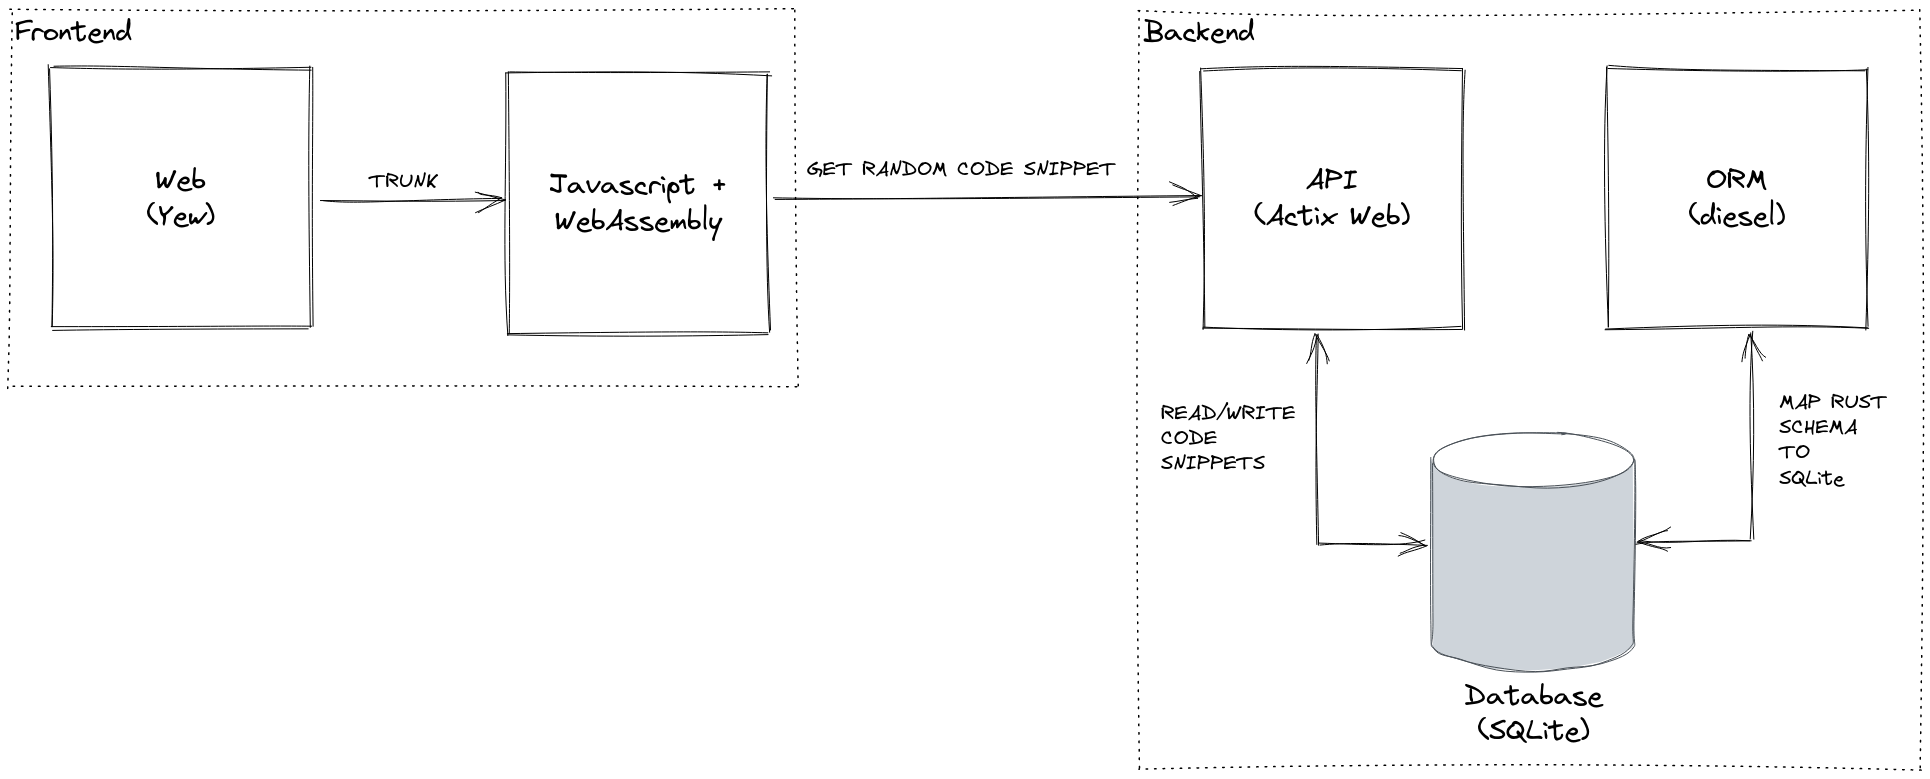
\includegraphics[width=\textwidth]{./figures/structuur.png}

De frontend van de applicatie is volledig geschreven in Rust. Dit is mogelijk gemaakt door het
gebruik van Yew als framework. Daarbij is er Tailwindcss gebruikt als CSS framework. Tailwindcss is
een utility-first CSS framework om snel custom user interfaces te bouwen. Samen met een component
based framework als Yew hoeven we zelf geen CSS meer schrijven maar kunnen we direct tailwindcss
zijn utility classes toepassen op mijn components. Wat maakt voor een geweldige developer
experience. 

Om alles van frontend te kunnen compileren en uitvoeren is er trunk gebruikt. Trunk is een WASM web
applicatie bundelaar. Het gebruikt een eenvoudige config voor het bouwen en bundelen van WASM, JS
snippets en andere assets (images, css, scss) via een source HTML bestand. Met een simpel commando
als \mintinline{bash}{trunk build} bouwt hij de hele frontend en met \mintinline{bash}{trunk serve
--open} draait hij een lokale dev server.  

Bij het laden van de startpagina haalt de frontend een willekeurig code fragment op via de API. De
API haalt de fragmenten op uit een SQLite database. Om de database in sync te houden met de Rust
code werd er diesel gebruikt als ORM framework.


\clearpage

\section{Werking frontend}

De startpagina is geïnspireerd door mijn favoriete editor vim. Zo krijgt u een simpele versie van
vim te zien als editor voor het typen. Hieronder ziet u een schema van de compositie van de
belangrijkste componenten.

\begin{figure}[h]
  \centering
  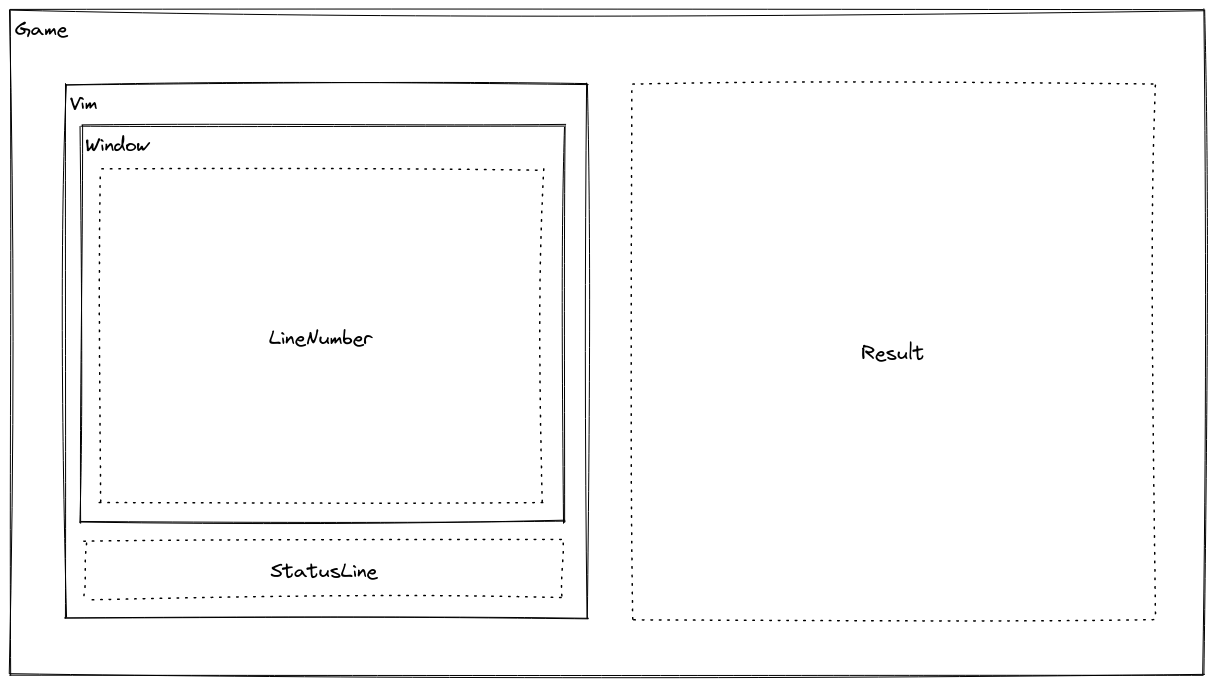
\includegraphics[width=0.9\textwidth]{./figures/components.png}
\end{figure}

\mintinline{rust}{Game}: rendert op basis van de game status \mintinline{rust}{Vim} of
\mintinline{javascript}{Result} 

\mintinline{rust}{Vim}: de tekst editor voor de code en bevat \mintinline{rust}{Window} \&
\mintinline{rust}{StatusLine} als children 

\mintinline{rust}{Window}: rendert de tekst samen met \mintinline{rust}{LineNumber} 

\mintinline{rust}{StatusLine}: toont live statistieken zoals de huidige taal, tijd, WPM, progress 

\mintinline{javascript}{Result}: toont alle statistieken op het einde van de game

Het bouwen van de interface was redelijk eenvoudig, maar om de speed typing test te doen werken was
het verassend moeilijk. Het duurde enkele iteraties tot de logica goed zat. Om de gebruiker het idee
te geven dat hij tekst over typt zijn er vier html elementen gebruikt: een cursor met het huidige
karkater, de correct getypte tekst, de foute getypte tekst en de resterende tekst.

\begin{wrapfigure}{l}{0.55\textwidth}
  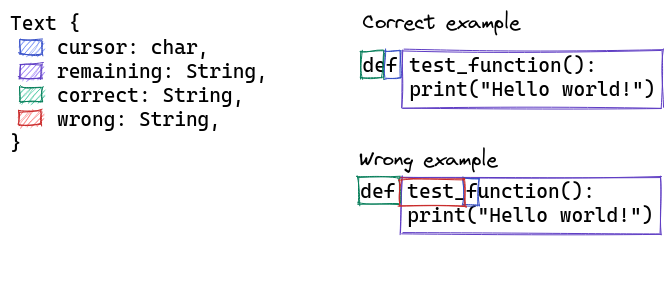
\includegraphics[width=\linewidth]{./figures/text.png}
\end{wrapfigure}

Bij elk keypress event wordt er gecontroleerd of de key gelijk is aan het volgende karakter. Indien
het gelijk is wordt het huidige karakter van de cursor toegevoegd aan de string met de correcte
karakters en de cursor schuift een karakter op. Hetzelfde geldt als men een verkeerde key indrukt
maar de cursor wordt dan toegevoegd aan de string met de foutieve karakters. Als de gebruiker de
“Backspace” toets indrukt kan hij zijn foute karakters verwijderen tot de string leeg is. 

\clearpage

Dit was het basisidee, de moeilijkheid van het bouwen lag vooral aan hoe we efficiënt de variabelen
van de tekst en de bijhorende statistieken in een state kunnen opslaan zodat elk component slechts
rendert als het nodig is.  

Mijn eerste oplossing was het gebruik van globale state met de \mintinline{rust}{use_reducer} hook.
Als u vertrouwd bent met React zijn de meeste hooks zoals \mintinline{rust}{use_reducer},
\mintinline{rust}{use_state}, \mintinline{rust}{use_effect} overgenomen in Yew. Indien niet leg ik
het kort even uit. Om simpele variabelen op te slaan in een state zoals bijvoorbeeld een boolean
gebruikt u de \mintinline{rust}{use_state} hook. Die zorgt ervoor dat de boolean doorheen het
component lifecycle hetzelfde blijft tenzij u hem aanpast. Als u hem aanpast dan zal het component
opnieuw renderen.  

De \mintinline{rust}{use_reducer} hook werkt gelijkaardig maar wordt gebruikt voor complexere
states. Zo komt het met een dispatch functie die een argument neemt van het type Action. Wanneer
deze wordt aangeroepen, worden de actie en de huidige waarde doorgegeven aan de reducer functie die
een nieuwe state berekent en retourneert.

Zo heb ik 5 acties gedefinieert: \mintinline{rust}{NewSnippet}, \mintinline{rust}{Keypress},
\mintinline{rust}{Backspace}, \mintinline{rust}{Tick} en \mintinline{rust}{Reset}. In die acties zit
de meeste logica van het spel en kan gebruikt worden in components om de state van het spel aan te
passen. 

\begin{figure}[h]
\centering
\begin{minipage}{.45\textwidth}
\begin{minted}{rust}
pub struct Code {
  pub lines: usize,
  pub cursor: Option<char>,
  pub remaining: String,
  pub correct: String,
  pub wrong: String,
}

pub struct Stats {
  pub progress: u8,
  pub mistakes: u8,
  pub wpm: u8,
  pub accuracy: u8,
  pub time: u8,
  pub combos: u8,
}
\end{minted}
\end{minipage}%
\begin{minipage}{.45\textwidth}
\begin{minted}{rust}
pub struct GameState {
  pub code: Code,
  pub stats: Stats,
  pub status: Status,
  pub language: String,
}

pub enum Action {
  NewSnippet(Snippet),
  KeyPress(char),
  BackSpace,
  Tick,
  Reset,
}


\end{minted}
\end{minipage}
\end{figure}

Het probleem met de \mintinline{rust}{use_reducer} hook is dat een component de hele state opneemt.
Als de child components een variabel nodig hebben van de state, moeten die als properties worden
doorgeven. Hier is niks mis mee tenzij u een diep genest child component hebt die afhankelijk is
van de state. Dan heeft u “prop drilling” waarbij u vanuit de parent component de props moet
doorgeven aan zijn children die dezelfde props dan doorgeven aan hun children, en zo verder tot dat
je bij de gewenste component bent.

\clearpage

\begin{figure}[h]
  \centering
  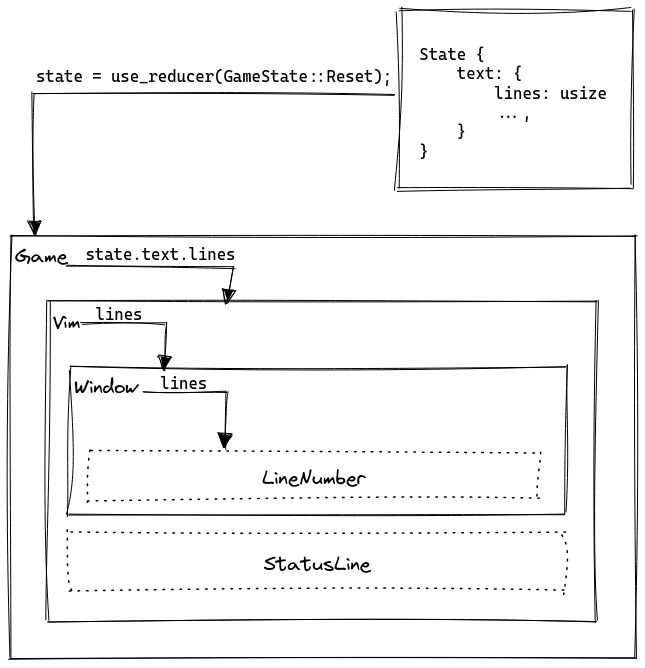
\includegraphics[width=0.6\textwidth]{./figures/use_reducer.png}
\end{figure}

Dit werd opgelost door de \mintinline{rust}{use_context} hook te gebruiken samen met de
\mintinline{rust}{use_reducer}. Zo kunnen we een \mintinline{rust}{GameStateProvider} component
definiëren die de context (state) consumeert en gebruikt kan worden door alle child components. Dit
betekent dat we de props niet meer hoefde te 'prop drillen' maar direct kon aanspreken vanuit alle
child components onder de \mintinline{rust}{GameStateProvider}. Helaas heeft deze methode ook zijn
nadelen: 
\begin{itemize}
    \item Als de state gebruikt wordt in een child component moet de hele state gekloond worden 

    \item Stel een child component gebruikt een variabele A van de globale state, als de hele state
    wordt aangepast behalve de variabele A zal het child component toch onnodig re-renderen 
\end{itemize}

Uiteindelijk is er de switch gemaakt naar yewdux, een state management library voor Yew die werkt
met een globale store/state. Het is verglijkbaar met de populaire React library Redux. Yewdux
gebruikt een CoW (clone on write) managementstrategie. Dit betekent dat de state bij elke mutatie
een keer wordt gekloond. Door het op deze manier te doen kunnen we beknopt een precieze mutatie
uitdrukken zonder extra boilerplate, en gebruik maken van change detection om onnodige re-renders te
voorkomen. 

Een voorbeeld hiervan is de \mintinline{rust}{use_selector} hook van yewdux, waarmee we een
variabele van de state kunnen selecteren en slechts re-renderen als de variabel verandert i.p.v. de
hele state.

\clearpage

\section{Werking backend}

De werking van de backend verschilt niet veel met het voorbeeld 'Todo' applicatie die we gemaakt
hebben in \enquote{Hoe bouwt u een API in Rust?}. Opnieuw werd er gekozen voor een simpele SQLite database
om de code snippets in op te slaan. Zoals eerder gezien wordt het database schema aangemaakt door
migrations uit te voeren met diesel CLI.  Dit is een database first aanpak, na wat onderzoek lijkt
het me dat diesel.rs jammer genoeg geen andere aanpakken ondersteund zoals code first. Met code
first kan u vanuit models die gedefinieerd staan in code automatisch migrations aanmaken die het
database schema aanpassen/aanmaken. 

In de speed typing database gebruiken we twee tabellen “languages” en “snippets”. Die een een op
veel relatie met elkaar hebben. De tabel languages bevat de soorten programmeertalen en de tabel
snippets de code. De code is hier gewoon opgeslagen als tekst in de tabel snippets. Het is wel
belangrijk dat de code geen spaties bevat maar tabs. Daarvoor is er kleine parser tool geschreven om
makkelijk code snippets te maken. Het neemt een tekstbestand als input en zet alle spaties en enters
om naar de respectievelijke karakters “\textbackslash t” en “\textbackslash n”. Zo kan de frontend
makkelijk de juiste enters en tabs weergeven. 

De API kent een aantal routes:
\begin{itemize}
    \item GET, POST, DELETE  /languages
    \item GET, POST, DELETE /snippets 
    \item GET /snippets/random 
    \item GET /snippets/\{language\_id\}"
\end{itemize}

Uiteindelijk gebruikt de frontend maar een route “/snippets/random” om een random code snippet op te
halen uit de database. 

Om ervoor te zorgen dat we niet eerst alle snippets op halen uit de database om dan een random
snippet eruit te selecteren. Wordt er eerst via een SQL-query de snippets tabel random gesorteerd en
het eerste resultaat eruit gepakt. Standaard zal Rust of diesel het random type niet kennen.
Gelukkig voorziet diesel de \mintinline{rust}{no_arg_sql_function} macro waarmee u SQL functies
kunt mappen naar Rust types.

\begin{listing}[h]
\begin{minted}{rust}
no_arg_sql_function!(
  random,
  sql::types::Integer,
  "Represents the SQL RANDOM() function"
)
\end{minted}
\end{listing}

Zo kunnen we het random type importeren vanuit het schema en gebruiken in mijn SQL-query opgesteld
door diesel.

\chapter{Reflectie}
\label{reflectie}

Het doel van de module 'Research Project' was om onderzoek te doen naar de vraag "Wat is de huidige
status van Rust voor het bouwen van webapplicaties?". In dit hoofdstuk reflecteer ik op het
resultaat van het onderzoek en vergelijk de bevindingen uit de praktijk. Daarvoor heb ik contact
opgenomen met twee core maintainers van het gebruikte web framework genaamd Yew. Zij hebben beide
ook professionele ervaring met het bouwen van webapplicaties in Rust.

De eerste core maintainer is Julius Lungys, hij is een Rust developer bij het Fintech bedrijf
Nikulipe. Al hun software is geschreven met Rust, de software is voornamelijk backend gericht maar
voor de admin websites gebruiken ze Yew. Julius was ook te gast bij \citetitle{podcast}
\cite{podcast} met een episode over Yew, waar ik interessante inzichten gekregen heb over dit
onderzoek.

Cecile Tonglet is de tweede core maintainer, in het dagelijkse leven ook een Rust developer
bij HMI Hydronics. Ze maken hydraulische ventielen, inclusief een "slimme" ventiel met wat embedded
code. Cecile werkt niet aan de niet aan de embedded software maar werkt aan een web app die draait 
op het slimme ventiel.

Naast de core maintainers heb ik ook gereflecteerd met Emiel Van Severen, een mastersstudent
Industrieel Ingenieur in de Informatica. Hij heeft nog geen professionele ervaring met Rust maar
is zich zeer bekend in het ecosysteem en heeft een aantal hobby projecten in Rust.

Ook was er tijdens het onderzoek ook aardig wat feedback van de Yew community. Yew heeft een
relatief kleine maar zeer actieve community. Zo kreeg ik in hun discord instant feedback bij
problemen of vragen.

\clearpage

\section{Wat zijn de sterke en zwakke punten van het resultaat uit jouw researchproject?}

\subsection{Sterke}

Tijdens het interview met Julius Lungys, stelde ik vraag waarom hij zo enthousiast is over Rust. 
Hij antwoorde dat de taal alles heeft wat hij wilt, een eigen equivalent van npm (Cargo), ingebouwde
code formatter, tests, docs, geen garbage collector en macros.

Dit kon ik alleen maar beamen, Cargo is een geweldige package manager en maakt het beheren van
packages zeer eenvoudig. Cargo is ongetwijfeld een van Rust zijn sterkte punten en zal een positieve
impact hebben op de groei van het ecosysteem.

Rust is correct met een krachtig typesysteem, dit betekent dat alle edge cases in de code worden
opgevangen. Denk maar aan het unwrappen van een \mintinline{rust}{Option} of
\mintinline{rust}{Result} type. Gelukkig heeft Rust een intelligente compiler die suggesties geeft
wanneer er iets fout loopt tijdens het compileren. Dit zorgt ervoor als de applicatie compileert, je
zeker kan zijn dat de meest voorkomende bugs er uit zijn.

In deelvraag \ref{productie} \enquote{Is Rust productie klaar?} zagen we dat de taal uitstekend
presteert bij de benchmarks zowel bij de frontend als backend. Als we de frontend resultaten
vergelijken met de populaire Javascript frameworks zien we dat Rust efficiënter omgaat met het
geheugen. Wat natuurlijk ook logisch is sinds Javascript een dynamische getypeerde taal is en
gebruik maakt van een garbage collector wat zorgt voor veel overhead. Samen met WebAssembly opent
dit de deuren om rekenkrachtige applicaties op het web te draaien die ervoor niet mogelijk waren.

\subsection{Zwakke}

Momenteel is het groottste nadeel het beperkte ecosysteem bij het bouwen voor de frontend van
webapplicaties. Hoe sneller een bedrijf een web app kan uitbrengen hoe minder kosten ze hebben. Dat
is een van de redenen waarom er bijvoorbeeld veel voorgestijlde component libraries op de markt zijn
voor Javascript. Yew voorziet al een paar copies van zo'n bekende Javascript libraries maar die zijn
allemaal nog te jong om te kunnen gebruiken in productie.

Samen met Rust is WebAssembly nog jong en volop in beweging. Zoals besproken in de deelvraag
\ref{productie} \enquote{Is Rust productie klaar?} is wasm nog niet perfect. Zo hoeven we nog altijd
javascript te gebruiken om te praten met de DOM, maar dit is slechts tijdelijk.

Voor dat Julius aan zijn Rust carrière begon was hij een React developer. Wat hem nu stoort is de
hoeveelheid boilerplate code dat je nodig hebt in Rust om het zelfde te kunnen bereiken in React.
Zo hoeven we bijvoorbeeld voor simpele functies aan te spreken in Javascript libraries gebruiken als
\mintinline{rust}{gloo} een high level wrapper rond de \mintinline{rust}{wasm-bindgen} crate die
speelt als 'lijm' tussen Rust en Javascript.

\clearpage

\section{Is ‘het projectresultaat’ (incl. methodiek) bruikbaar in de bedrijfswereld?}

Kort gezegd, ja. De technische demo toonde aan welke stappen er ondernomen moesten worden voor een
simpele webapplicatie te bouwen. Deze stappen kunnen we beschouwen als een basis die een bedrijf kan
gebruiken voor een webapp te bouwen in Rust. De methodiek werd dan ook afgetoetst bij externen.
Julius en Cecile hadden beide geen opmerkingen over de structuur/methodiek van het project. 

Julius gebruikt zelf een gelijkaardige structuur in de praktijk. Op zijn werk gebruiken ze een grote
mono repo waar all hun services inclusief de web applicaties inzitten. Met als voordeel dat ze een
paar crates hebben met code die ze kunnen delen, bijvoorbeeld een crate database entiteiten.

\section{Wat zijn de mogelijke implementatiehindernissen voor een bedrijf?}

De huidige stabel release van Yew heeft nog geen SSR. Dit betekent met de huidige CSR, er twee grote
nadelen zijn:
\begin{itemize}
   \item Gebruikers zullen niets kunnen zien totdat de hele WebAssembly bundel is gedownload en de
   eerste render is voltooid. Dit kan resulteren in een slechte gebruikerservaring als de gebruiker
   een traag netwerk gebruikt.

  \item Sommige zoekmachines ondersteunen geen dynamisch gerenderde web content en zij die dat wel
  doen plaatsen dynamische websites meestal lager in de zoekresultaten.
\end{itemize}
Het gebrek aan SSR kan dus gezien worden als een implementatiehindernis, indien het bedrijf zijn web
app wil optimaliseren.

Een andere implementatiehindernis kan zijn dat het team binnen het bedrijf geen ervaring heeft met
Rust. De taal opzich heeft al een steile leercurve, daarnaast moeten ze ook nog bedrijpen hoe
WebAssembly werkt. Gelukkig hebben mensen met React ervaring al een voorsprong als ze voor het Yew
framework kiezen, sinds het bijna een excate copie is.

\section{Wat is de meerwaarde voor het bedrijf?}

Als een bedrijf de frontend van een applicatie volledig in Rust schrijft, zal dat op dit moment niet
veel meerwaarde brengen. Buiten dat als een bedrijf een volledige stack heeft in Rust, ze het
makkelijk kunnen vinden om ook hun web applicaties ook te bouwen in Rust. 

Zoals besproken in sectie \ref{productie} \enquote{Is Rust productie klaar?} is de grootste use case
momenteel om Rust/WebAssembly te gebruiken waar er grote prestatie vereisen zijn of een gedeelte van
de applicatie als de logica in Rust schrijven.

Wat wel interessant is, is om micro services te schrijven in Rust die we kunnen gebruiken voor het
web. Rust zijn binary grootte zonder te compileren naar WebAssembly is klein. Daarnaast is Rust ook
super snel, perfect voor kleine micro services in de cloud. Denk maar bijvoorbeeld aan AWS lambda
functies. Emiel weette mij te vertellen dat nu ook Cloudflare workers volledig in Rust geschreven
kunnen worden. \cite{cloudflare_workers}

Ten slotte is het niet onbelangrijk om te vermelden dat Rust ondertussen al 6 jaar op een rij als de meest
geliefde taal bij een enquête van Stack Overflow. \cite{so_enquete} 

\section{Welke suggesties geven bedrijven en/of community?}

Wanneer ik aan het zoeken was naar externen om te reflecteren, had ik een bericht geplaatst in de
Yew discord server. Daar kreeg ik ook feedback. Zij stelden voor om de wasm code bij de server te
comprimeren, zodat het niet de client ~380kB aan wasm code ongecomprimeerd laat downloaden over het
internet. Een andere suggestie van de community was om de \mintinline{rust}{reqwasm} crate te laten
vallen, want die is ondertussen toegevoegd aan de \mintinline{rust}{gloo} crate. Dit zou ook de wasm
binary grootte kunnen verkleien.

Emiel suggesteeerde om testen te schrijven, Rust heeft daarvoor een heel goed builtin test systeem.
Dat had zeker een meerwaarde kunnen zijn om bijvoorbeeld de parser tool uit te werken met behulp van
test driven development.

Julius stelde ook voor om de \mintinline{rust}{hooks} te gebruiken van \mintinline{rust}{Trunk}, op
die manier zou ik een hook kunnen schrijven die bij het bouwen van de applicatie ook de tailwindcss
scripts uitvoert. De huidige manier was via een npm script.

\section{Wat zijn jouw suggesties voor een (eventueel) vervolgonderzoek?}

Vooraleer ik aan het research project begon, werd er gevraagd een contractplan in te vullen. 
Daarin had ik een opsomming opgelijst van wat het resultaat van mijn technisch onderzoek minimaal
zal bevatten. Helaas heb ik tijdens het onderzoek de tijd niet gehad voor alles te realiseren. 
Ik lijst hier even kort op welke criterea's ik niet heb kunnen realiseren:
\begin{enumerate}
  \item De applicatie is beveiligd met SSO
  \item Er is een profiel pagina aanwezig
  \item De statistische resultaten worden opgeslaan in een database
\end{enumerate}
In een vervolgonderzoek zou ik de applicatie dan ook uitbreiden met deze functionaliteiten. Om de
applicatie te beveiligen met SSO, zou ik OAUTH implementeren. Op die manier kunnen gebruikers
inloggen met bijvoorbeeld hun Github account.  Met een gebruikers account zal ik ook een profiel
pagina kunnen aanmaken en de statistische resultaten per gebruiker opslaan in de database.

Tijdens het onderzoek heb ik geen aandacht gegeven aan ci/cd. Ondertussen heb ik al een kleine
pipeline opgezet om de frontend te deployen naar een Azure Static Web App en de api naar een Azure
API App. Dit is vlug opgezet en kan zeker ook verder onderzocht / geoptimaliseert worden.

Wat ik ook nog niet heb onderzocht is het optimaliseren van de wasm binary.\cite{wasm_size} Volgens
de community zijn er een aantal stappen die je kan ondernemen om je binary te verkleinen. Wat
belangrijk is, want we hebben gezien bij de benchmark resultaten dat Yew een grotere bundle size
over het internet stuurt dan Javascript frameworks.

Als laatste zou ik proberen een javascript module als bijvoorbeeld \mintinline{javascript}{Chart.js}
gebruiken in het web project. Dit zou mogelijk moeten zijn door de \mintinline{rust}{wasm-bindgen}
crate te gebruiken om de functies van de JS library te mappen naar Rust. Met
\mintinline{javascript}{Chart.js} zou ik dan een grafiek kunnen tonen van de afgelopen resultaten.

\chapter{Lijst met afkortingen}

\chapter{Conclusie}

/chapter{Referenties}

\chapter{Bijlages}


\end{document}
